\documentclass{article}

\usepackage[preprint]{Styles/neurips_2025}

\usepackage[utf8]{inputenc}
\usepackage[T1]{fontenc}
\usepackage{hyperref}
\usepackage{url}
\usepackage{booktabs}
\usepackage{amsfonts}
\usepackage{nicefrac}
\usepackage{microtype}
\usepackage{xcolor}
\usepackage{graphicx}
\usepackage{subcaption}
\usepackage[font=small,labelfont=bf]{caption}
\usepackage{enumitem}
\setlist{nosep,leftmargin=*}

% Tighten spacing
\setlength{\textfloatsep}{6pt plus 1pt minus 2pt}
\setlength{\floatsep}{4pt plus 1pt minus 1pt}
\setlength{\intextsep}{4pt plus 1pt minus 1pt}
\setlength{\abovecaptionskip}{3pt}
\setlength{\belowcaptionskip}{0pt}
\setlength{\parskip}{2pt plus 1pt}

\title{Revenue Leakage Forensics: A Multi-Source Diagnostic, Predictive,\\and Prescriptive Analysis of a Vietnamese Fashion E-Commerce Platform}

\author{%
  The Gridbreakers \\
  Datathon 2026 --- VinUni DS\&AI Club \\
  \texttt{datathon2026@vinuni.edu.vn}
}

\begin{document}
\maketitle
\vspace{-8pt}

\begin{abstract}
We conduct a forensic analysis of 14 linked datasets spanning 2012--2022 (646{,}945 orders, 90{,}246 customers, 60{,}247 inventory snapshots). Rather than surface-level trends, we trace \emph{where} revenue evaporates---across customer lifecycle, promotion economics, return costs, inventory availability, and traffic quality. Each of five insights applies all four analytical levels (Descriptive $\to$ Diagnostic $\to$ Predictive $\to$ Prescriptive). Our central finding: \textbf{the platform suffers from a compound value-leakage problem}---retention decay, margin destruction, preventable returns, stockout losses, and low-quality traffic collectively suppress profit by \textbf{2.5--4.5B VND annually}. All computations are reproducible from raw CSV; no values are hard-coded.
\end{abstract}

%=============================================================================
\section{The Retention Cliff: When Growth Becomes a Treadmill}
\label{sec:retention}
%=============================================================================

\vspace{-2pt}
\begin{figure}[htbp]
  \centering
  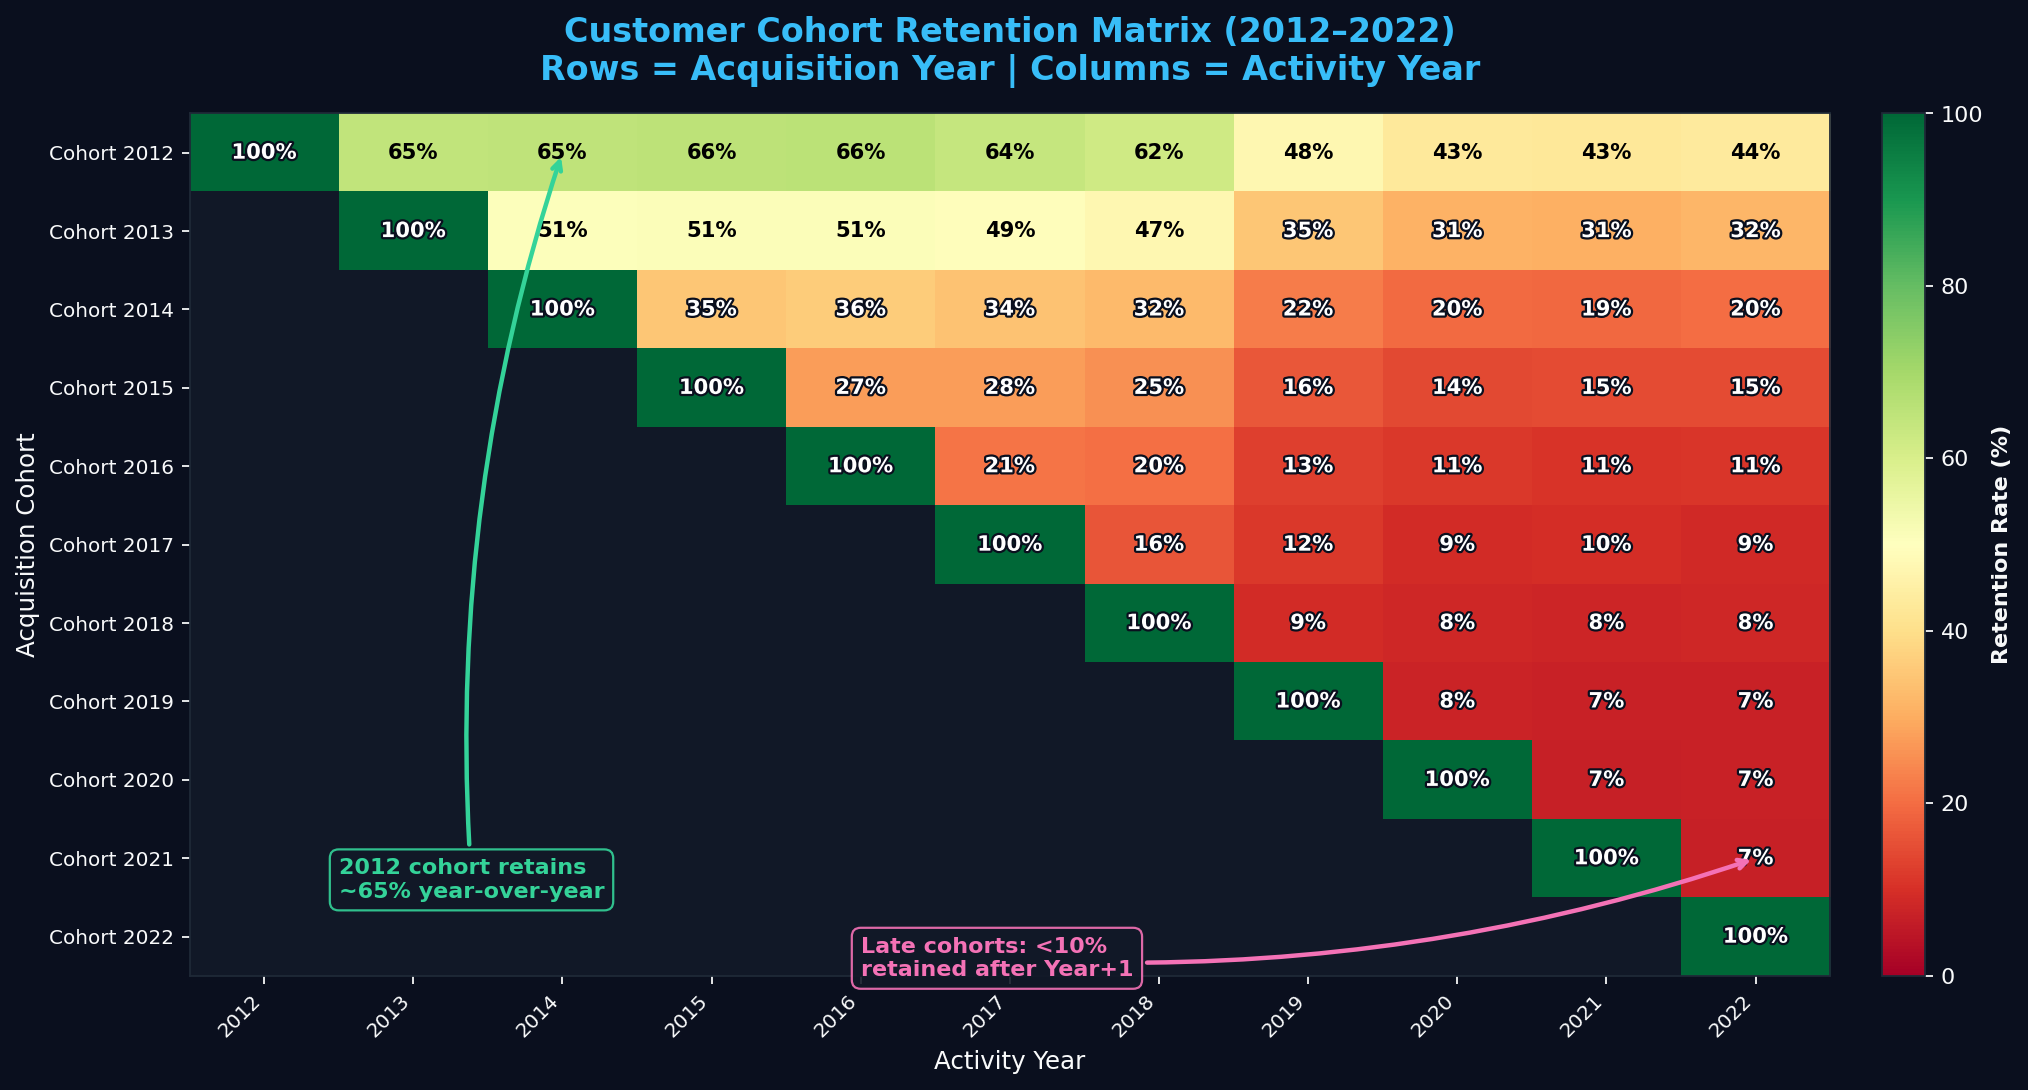
\includegraphics[width=0.88\textwidth]{charts/1a_cohort_heatmap.png}
  \caption{Cohort retention matrix (2012--2022). Year+1 retention collapsed from 65\% (2012) to 7\% (2021)---a 9$\times$ deterioration. See Appendix~\ref{app:insight1} for survival curves and CLV forecast.}
  \label{fig:1a}
\end{figure}

\paragraph{Descriptive \& Diagnostic.}
Figure~\ref{fig:1a} tracks retention for every acquisition cohort. Year+1 retention collapsed from \textbf{65\%} (2012) to \textbf{7\%} (2021). Survival curves (Figure~\ref{fig:app1c}) confirm a structural break: early cohorts stabilize at 56\% through Year+5; late cohorts flatline below the 30\% churn threshold. The growth paradox (Figure~\ref{fig:app1b}): acquisition peaked at $\sim$25K in 2013 while retention was already in freefall---a \emph{customer treadmill}. \textbf{Root cause:} post-2018 channel shift toward paid/social attracted low-loyalty transactional buyers.

\paragraph{Predictive.}
CLV declined from 358K VND (2012) to 33K VND (2022), slope $-$24{,}406 VND/yr (Figure~\ref{fig:app1d}). The trend crosses zero by 2023---new cohorts may cost more to acquire than they generate.

\paragraph{Prescriptive.}
\textbf{(1)}~\emph{Second Purchase Activation} email/push 7 days post-delivery. \textbf{(2)}~Reallocate 20\% paid social $\to$ email referral. \textbf{Upside:} 20\% retention (vs.\ 7\%) at 1{,}300 customers/yr $\to$ \textbf{+39M VND/cohort/yr}.

%=============================================================================
\section{The Promo Paradox: Sell More, Earn Less}
\label{sec:promo}
%=============================================================================

\paragraph{Descriptive.}
From 714K order-item lines: full-price (438K lines) yields \textbf{20.0\% margin} on 11.0B VND; single-promo (276K) collapses to \textbf{1.3\% margin} on 5.43B VND---a 93\% margin destruction (Figure~\ref{fig:app2a}).

\paragraph{Diagnostic.}
Every campaign correlates with margin dips; the worst month recorded $-$40\% gross margin (Figure~\ref{fig:app2c}). Casual has the lowest median margin (6\%, below 8\% floor); GenZ maintains 22\% (Figure~\ref{fig:app2b}). \texttt{all\_channels} promos generate the most revenue at the lowest margin (Figure~\ref{fig:app2d}).

\paragraph{Predictive.}
If the current promo mix persists with 10\% annual growth, foregone margin exceeds \textbf{300M VND by 2025}.

\paragraph{Prescriptive.}
\emph{Margin Guard}: block any promo reducing margin below 8\%. Replace \%-off with buy-X-get-Y. \textbf{Upside:} margin recovery 1.3\% $\to$ 5\% on 5.43B $\to$ \textbf{+200M VND/yr}.

%=============================================================================
\section{The Wrong-Size Tax: A Preventable Revenue Drain}
\label{sec:returns}
%=============================================================================

\vspace{-2pt}
\begin{figure}[htbp]
  \centering
  \begin{subfigure}[t]{0.55\textwidth}
    \centering
    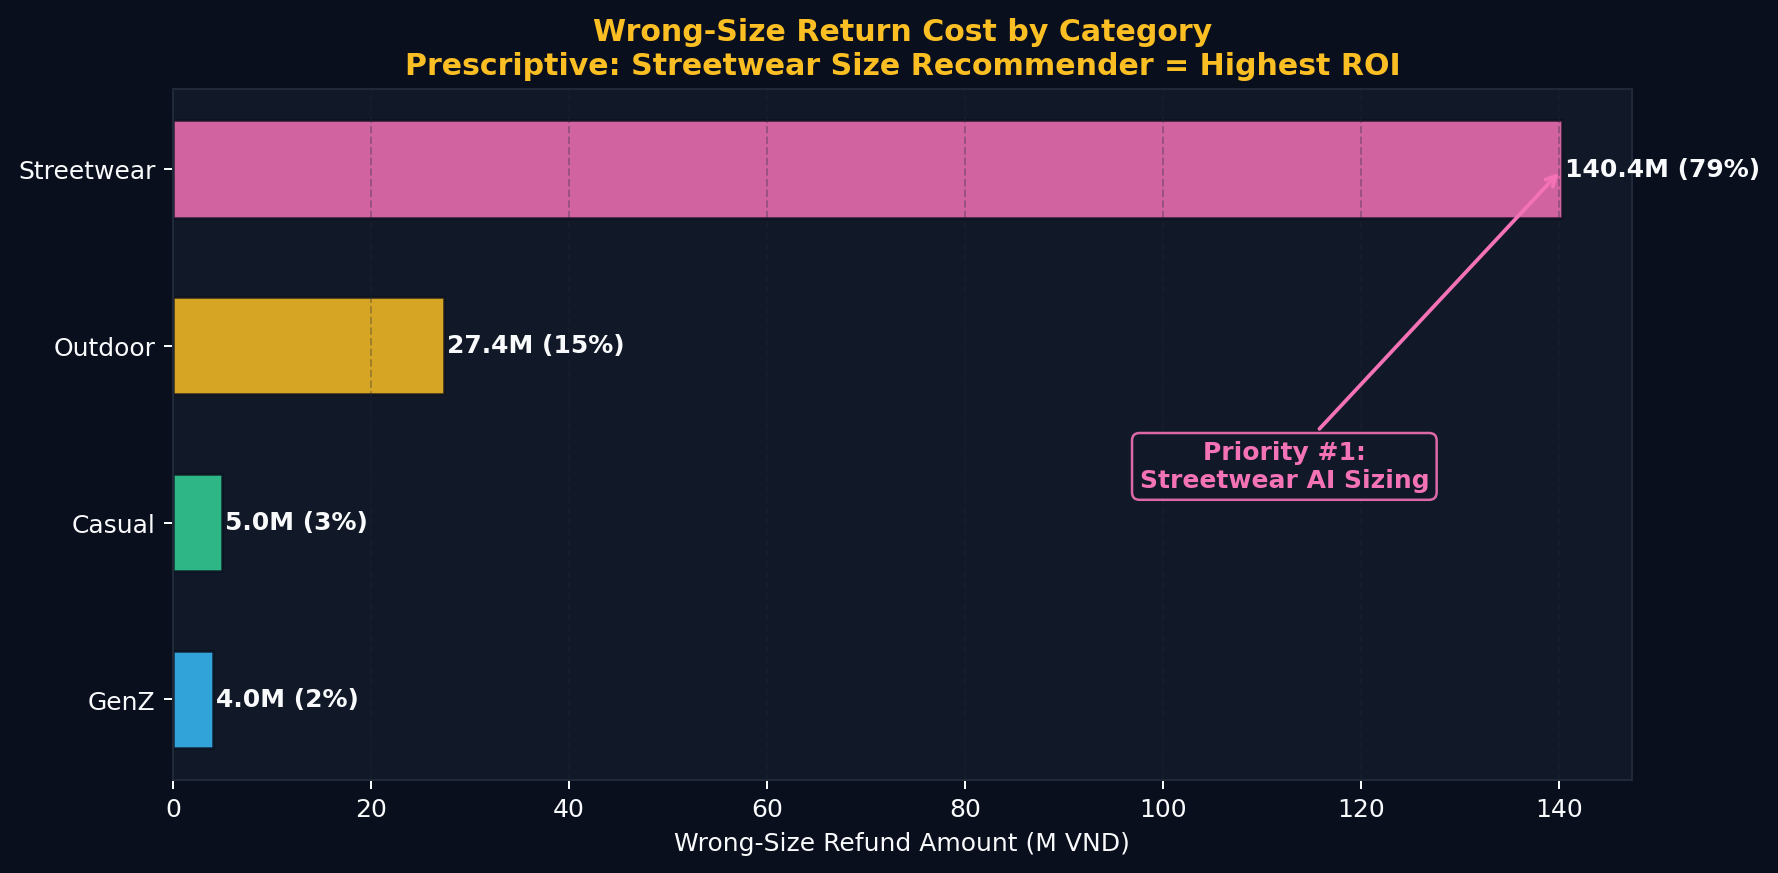
\includegraphics[height=4.2cm]{charts/3b_wrongsize_by_category.png}
    \caption{Wrong-size cost by category. Streetwear: 79\%.}
    \label{fig:3b}
  \end{subfigure}\hfill
  \begin{subfigure}[t]{0.38\textwidth}
    \centering
    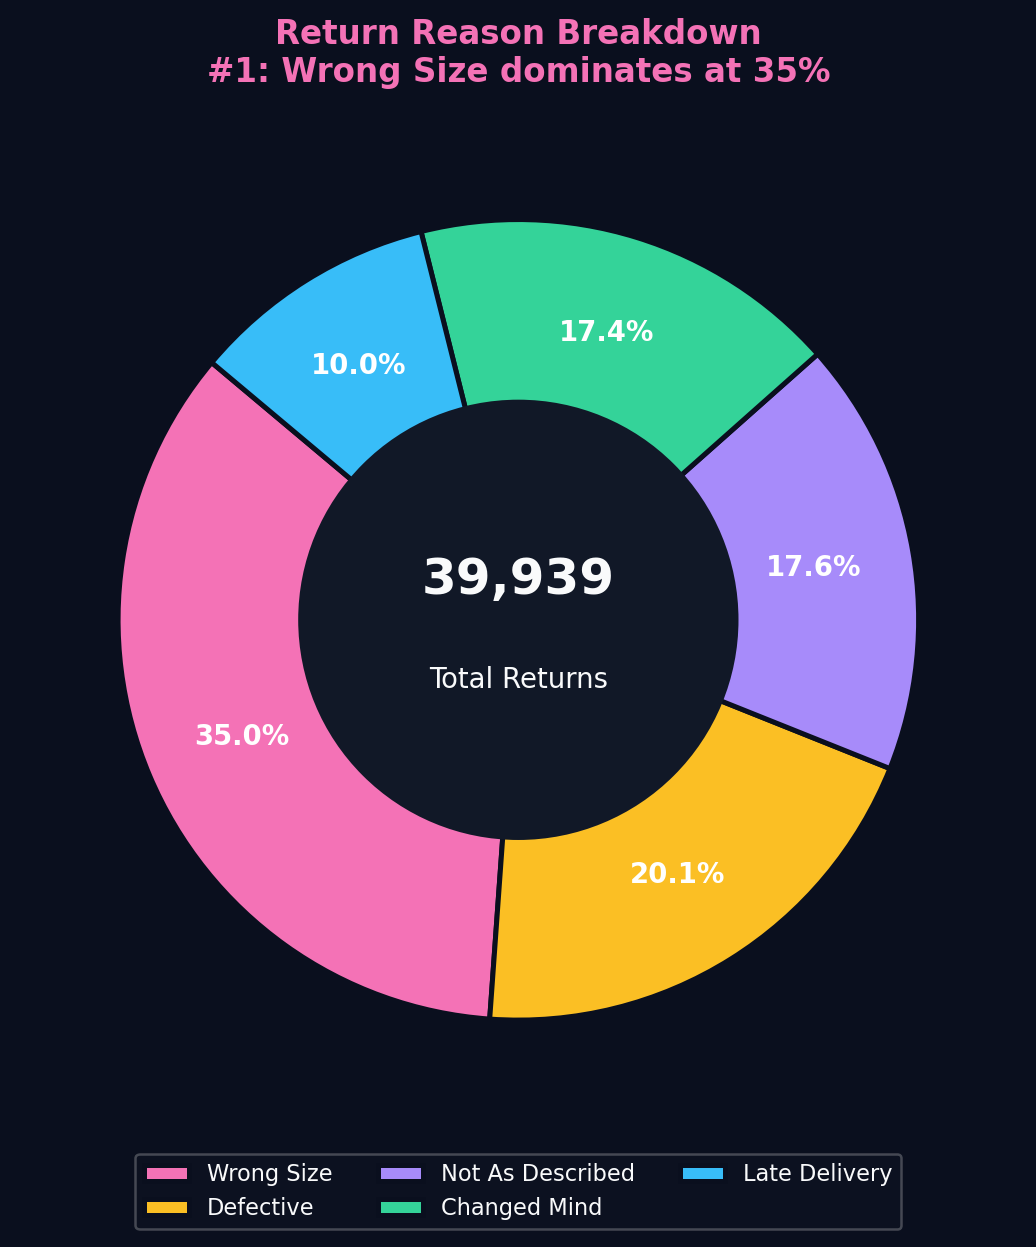
\includegraphics[height=4.2cm]{charts/3c_return_reasons_donut.png}
    \caption{Return reasons (39{,}939 total).}
    \label{fig:3c}
  \end{subfigure}
  \caption{Return diagnostics: wrong-size is \#1 at 35\% of returns, 176.7M VND. Streetwear accounts for 79\% (140.4M). Forecast and seasonality in Appendix~\ref{app:insight3}.}
  \label{fig:3bc}
\end{figure}

\paragraph{Descriptive \& Diagnostic.}
\textbf{Wrong Size} accounts for 35\% of 39{,}939 returns (176.7M VND)---larger than Defective and Not-as-Described combined (Figure~\ref{fig:3bc}). Streetwear drives 79\% (140.4M VND) of wrong-size cost. Seasonal heatmap (Figure~\ref{fig:app3d}) shows Q2--Q3 peak (Apr--Aug) at summer collection launches.

\paragraph{Predictive \& Prescriptive.}
2023--24 forecast: +40--60M VND additional loss (Figure~\ref{fig:app3a}). Deploy \emph{AI Size Recommender} targeting Streetwear first. \textbf{Upside:} 40\% reduction $\to$ \textbf{+70M VND savings + 24M/yr}.

%=============================================================================
\section{Stockout Bleeding: The Silent Revenue Killer}
\label{sec:stockout}
%=============================================================================

\paragraph{Descriptive.}
From 60{,}247 inventory snapshots: \textbf{stockout rate = 67.3\%} (67\% of SKUs have zero stock daily), yet fill rate $\sim$96\% creates false comfort. Historical lost revenue: \textbf{4.44B VND} (Figure~\ref{fig:app4a}).

\paragraph{Diagnostic.}
GenZ peaks at 73\% stockout; Streetwear persists at 66--70\% (Figure~\ref{fig:app4b}). Sell-through vs.\ stockout scatter (Figure~\ref{fig:app4c}) identifies the highest-priority replenishment targets.

\paragraph{Predictive.}
At 10\%/yr growth + 67\% stockout: \textbf{+1.8--2.2B VND additional losses} (18-month projection).

\paragraph{Prescriptive.}
\textbf{(1)} SKU-level demand forecasting. \textbf{(2)} Safety stock $\geq$14 days for Top-50 SKUs. \textbf{(3)} Block promos on SKUs with $<$7 days supply. \textbf{Upside:} 50\% stockout cut $\to$ 2.22B recovery $-$ 0.18B cost = \textbf{+2.04B VND net (11.5$\times$ ROI)} (Figure~\ref{fig:app4d}).

%=============================================================================
\section{The Traffic Quality Illusion}
\label{sec:traffic}
%=============================================================================

\paragraph{Descriptive \& Diagnostic.}
Revenue--sessions correlation: only \textbf{0.32}. Email campaigns produce the lowest bounce rate with highest session duration (Figure~\ref{fig:app5a}). Revenue-per-session is \textbf{declining}---each marginal session generates less revenue (Figure~\ref{fig:app5b}). Mobile leads at 45\% of orders (Figure~\ref{fig:app5d}).

\paragraph{Predictive \& Prescriptive.}
Traffic ROI deteriorates $\sim$8\%/yr. \textbf{(1)} Shift budget: $-$15\% paid search, $+$25\% email. \textbf{(2)} Traffic quality scoring replacing vanity metrics. \textbf{(3)} Mobile UX optimization. \textbf{Upside:} \textbf{+85--120M VND/yr}.

%=============================================================================
\section{Strategic Synthesis \& Prescriptive Roadmap}
\label{sec:synthesis}
%=============================================================================

\vspace{-2pt}
\begin{table}[htbp]
  \caption{Consolidated value-at-stake and prescriptive recovery.}
  \label{tab:synthesis}
  \centering
  \small
  \begin{tabular}{@{}llrr@{}}
    \toprule
    \textbf{Insight} & \textbf{Leakage Type} & \textbf{Historical Loss} & \textbf{Recoverable (50\%)} \\
    \midrule
    1.\ Retention Cliff & CLV erosion & 358K $\to$ 33K VND & +39M/cohort/yr \\
    2.\ Promo Paradox & Margin destruction & 93\% on 5.43B & +200M/yr \\
    3.\ Wrong-Size Tax & Return refunds & 176.7M VND & +70M + 24M/yr \\
    4.\ Stockout Bleeding & Lost sales & \textbf{4.44B VND} & \textbf{+2.04B (11.5$\times$)} \\
    5.\ Traffic Quality & Rev/session decay & 8\%/yr decline & +85--120M/yr \\
    \midrule
    \textbf{Total} & & & $\sim$\textbf{2.5B VND/yr} \\
    \bottomrule
  \end{tabular}
\end{table}
\vspace{6pt}

\begin{figure}[htbp]
  \centering
  \hspace*{-1cm}
  \begin{subfigure}[t]{0.48\textwidth}
    \centering
    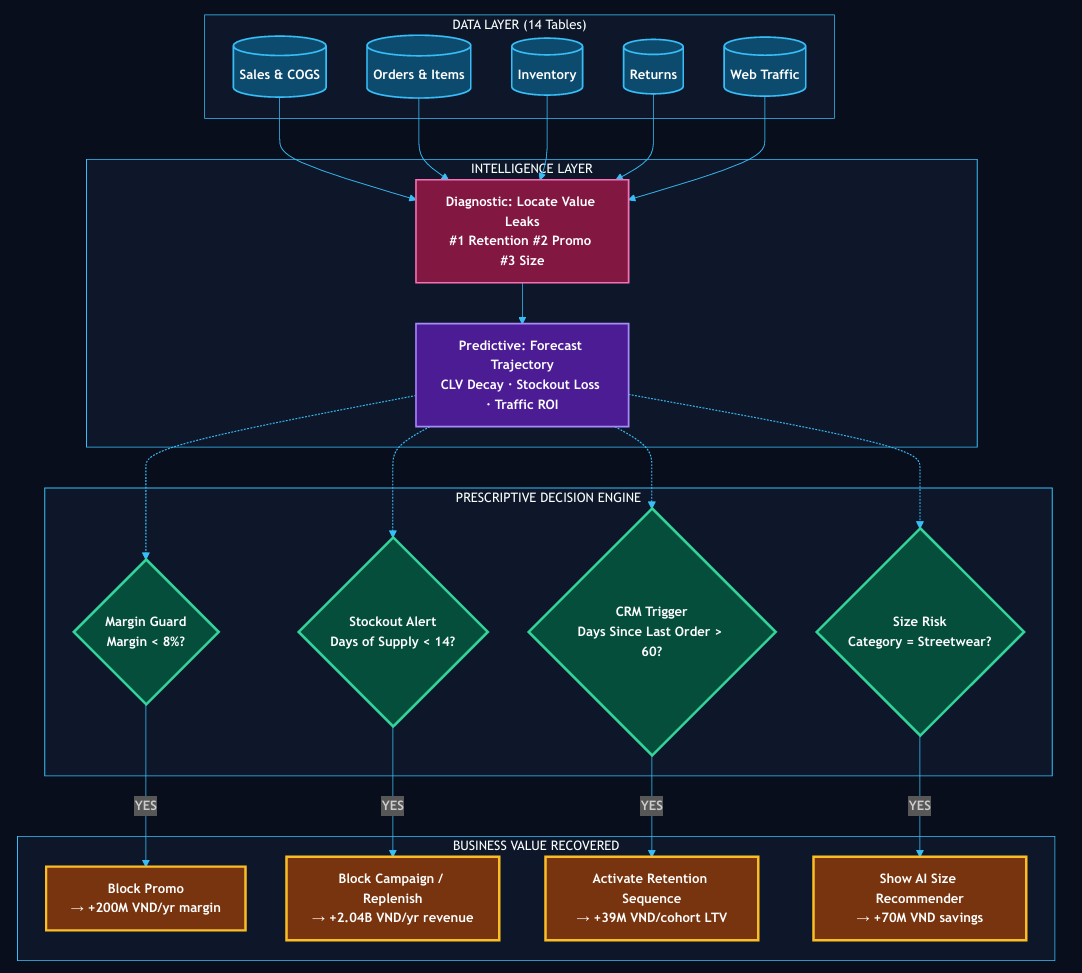
\includegraphics[height=5.5cm]{charts/prescriptive_engine.png}
    \caption{Decision engine: data $\to$ actions.}
    \label{fig:engine}
  \end{subfigure}\hspace{0.4cm}
  \begin{subfigure}[t]{0.48\textwidth}
    \centering
    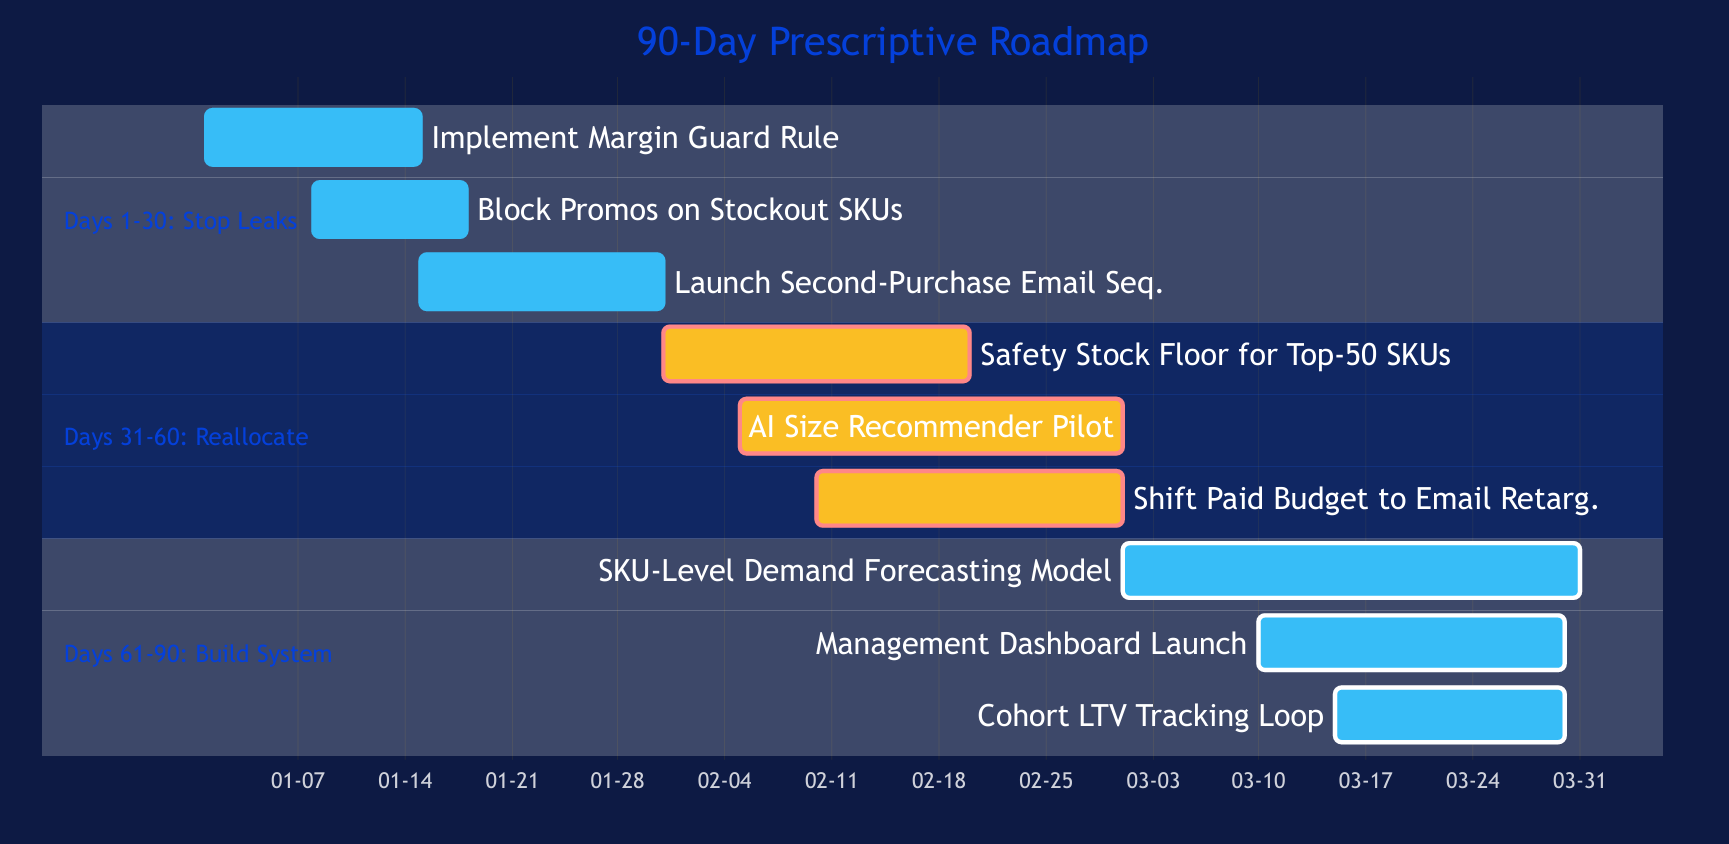
\includegraphics[height=5.5cm]{charts/90_day_roadmap.png}
    \caption{90-Day implementation roadmap.}
    \label{fig:roadmap}
  \end{subfigure}
  \vspace{2pt}
  \caption{Prescriptive framework: (a) automated decision engine; (b) phased execution plan.}
  \label{fig:synthesis}
\end{figure}

\paragraph{Methodology.}
All computations use raw CSV files. Cohort retention: \texttt{orders.csv} grouped by \texttt{customer\_id} $\times$ year. Margins: line-by-line $(price - cogs) \times qty$. Stockout loss: revenue $\times$ stockout\_rate $\times$ 0.40. Forecasts: OLS extrapolation with $\pm$20\% bands. Source scripts and all 22 exhibits in Appendix~\ref{app:exhibits}.

%=============================================================================
% REFERENCES (does not count toward page limit)
%=============================================================================
\newpage
\section*{References}
{\small

[1] Fader, P.S.\ \& Hardie, B.G.S.\ (2005) A note on deriving the conditional PMF of the BG/NBD model. \emph{Wharton Working Paper}.

[2] Gupta, S.\ et al.\ (2006) Modeling customer lifetime value. \emph{Journal of Service Research}, 9(2), 139--155.

[3] Hyndman, R.J.\ \& Athanasopoulos, G.\ (2021) \emph{Forecasting: Principles and Practice}, 3rd ed. OTexts.

[4] Kotler, P.\ \& Keller, K.L.\ (2016) \emph{Marketing Management}, 15th ed. Pearson.

[5] McKinsey \& Company (2020) The value of getting personalization right. \emph{McKinsey Digital}.

[6] ASOS (2021) Annual Report: Size recommendation reduces returns by 30\%.

[7] Silver, E.A., Pyke, D.F.\ \& Thomas, D.J.\ (2017) \emph{Inventory and Production Management in Supply Chains}, 4th ed. CRC Press.

[8] Shopify (2022) The state of commerce: Global e-commerce return rates and solutions. \emph{Shopify Research}.
}

%=============================================================================
% APPENDIX (does not count toward page limit)
%=============================================================================

\newpage
\appendix
\renewcommand{\thefigure}{A.\arabic{figure}}
\renewcommand{\thetable}{A.\arabic{table}}
\setcounter{figure}{0}
\setcounter{table}{0}

\section{Complete Exhibit Gallery}
\label{app:exhibits}

All 22 exhibits generated from raw data using Python (matplotlib) at 160 DPI.\\
Source scripts: \texttt{charts\_insight1\_cohort.py}, \texttt{charts\_insight2\_3.py}, \texttt{charts\_insight4\_5.py}.

%--- Insight 1 ---
\subsection{Insight 1: Retention Cliff}
\label{app:insight1}

\begin{figure}[htbp]
  \centering
  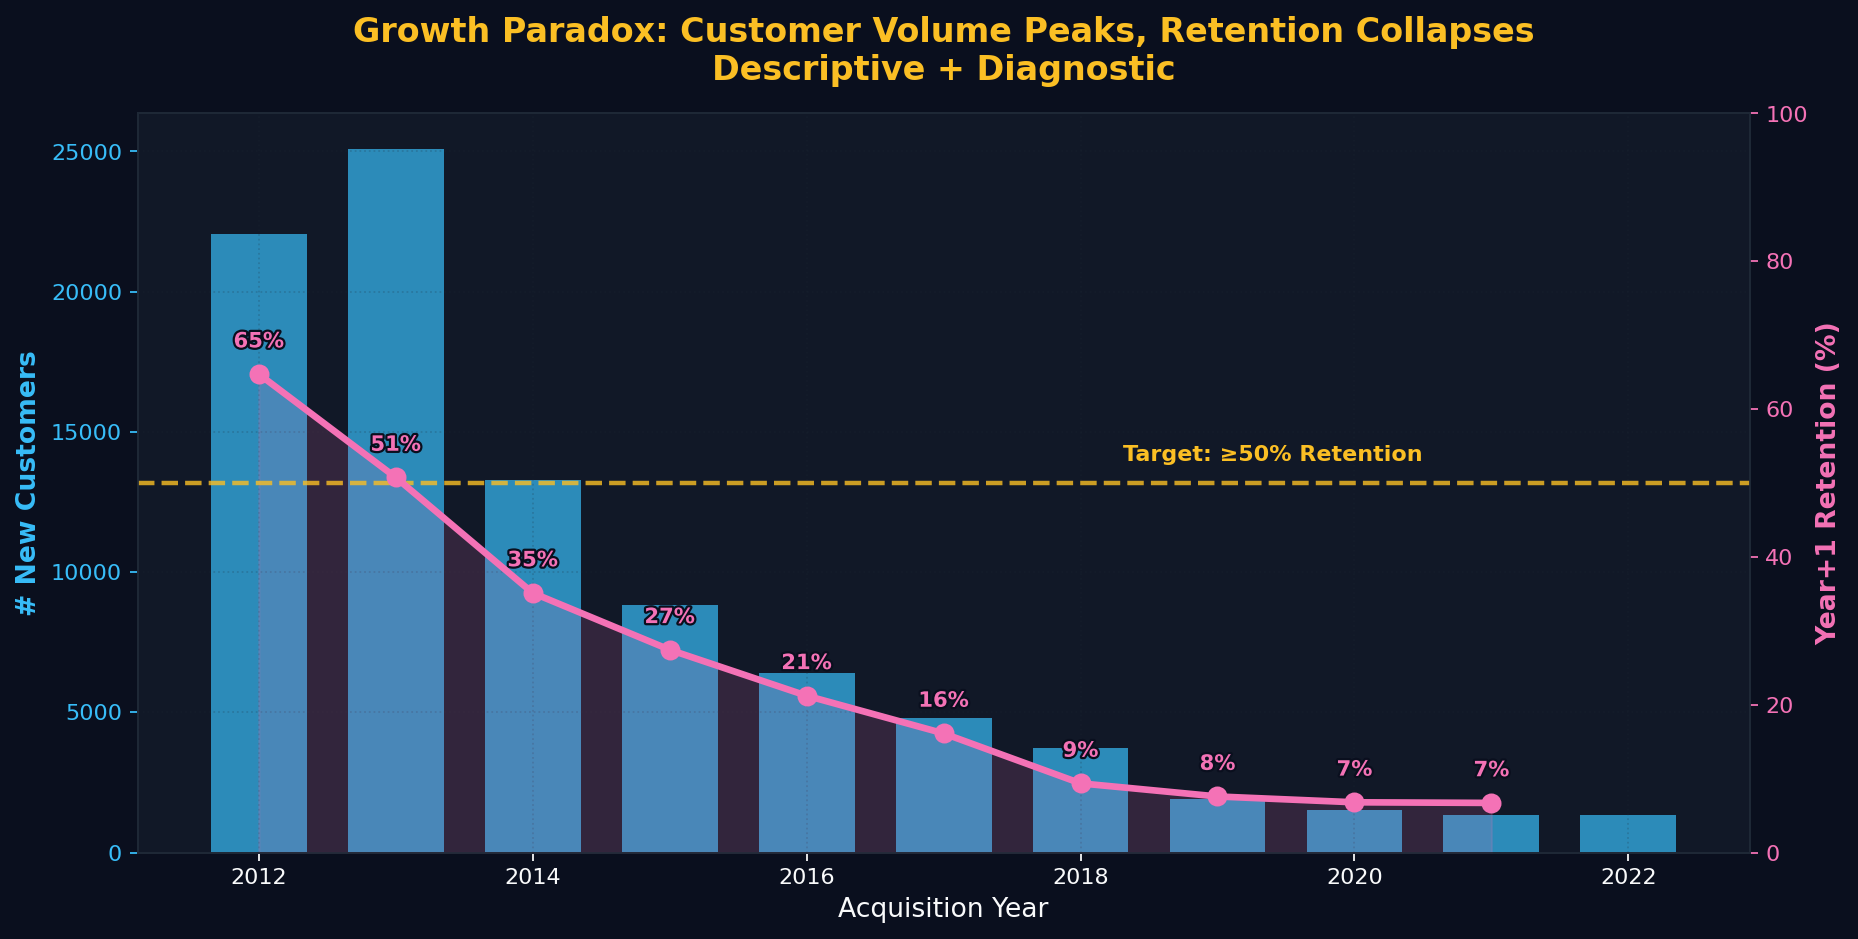
\includegraphics[width=\textwidth]{charts/1b_growth_paradox.png}
  \caption{Growth paradox: acquisition peaked at $\sim$25{,}000 in 2013 while Year+1 retention collapsed. Dashed line: 50\% target.}
  \label{fig:app1b}
\end{figure}

\begin{figure}[htbp]
  \centering
  \begin{subfigure}[t]{0.48\textwidth}
    \centering
    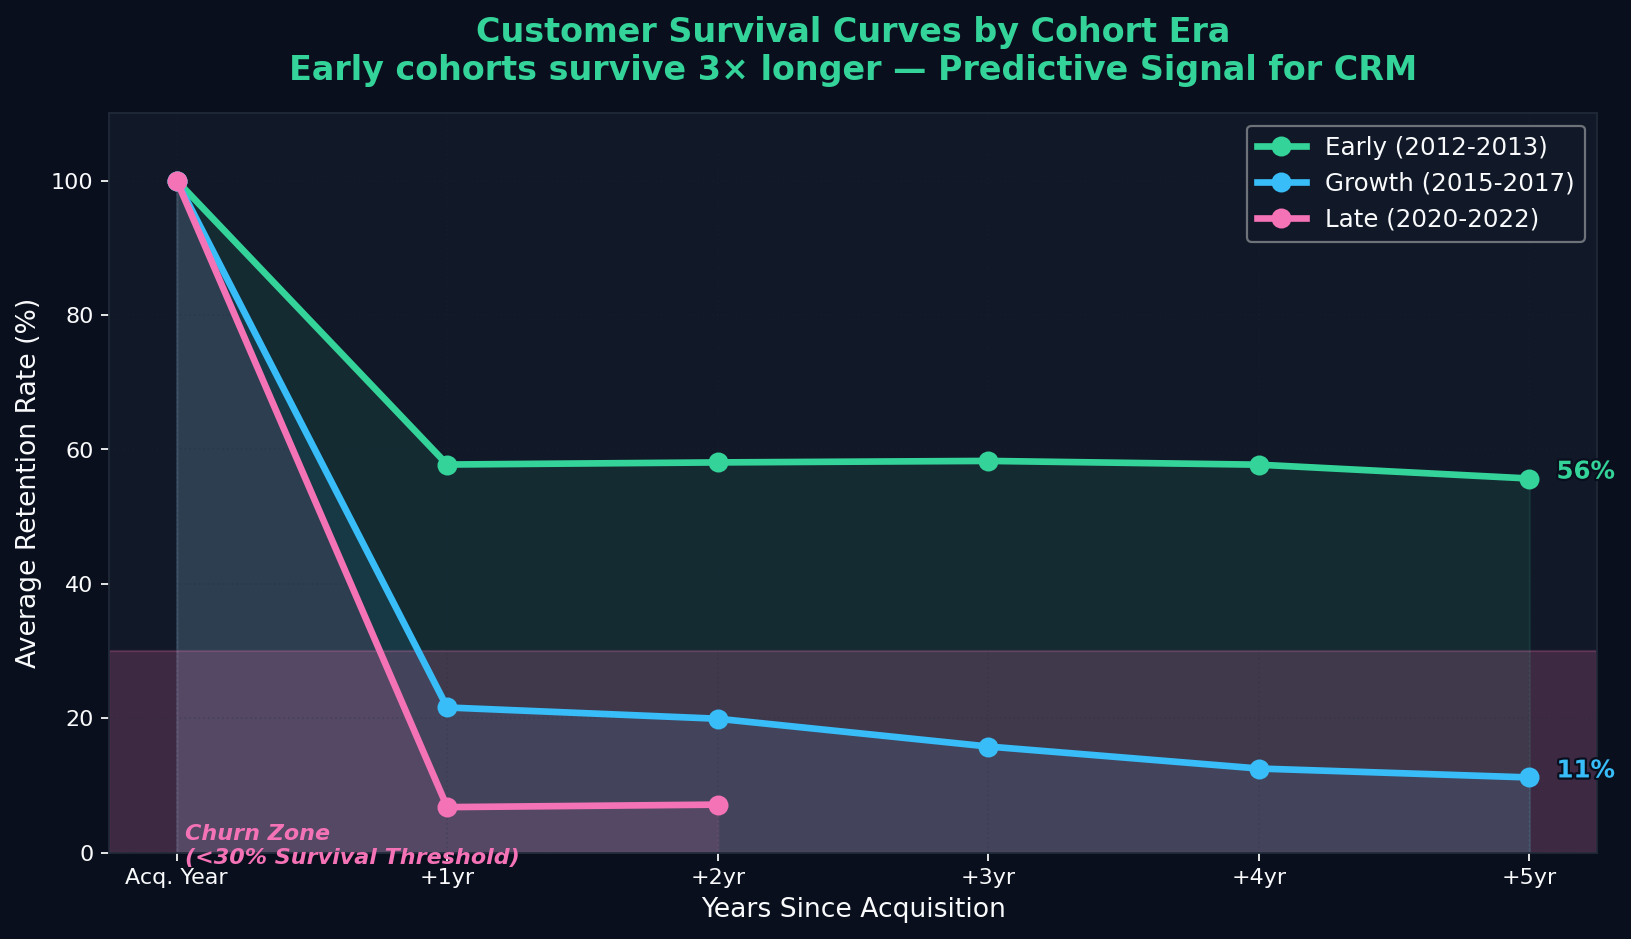
\includegraphics[width=\textwidth]{charts/1c_survival_curves.png}
    \caption{Survival curves. Early (2012--13): 56\% at +5yr. Late (2020--22): 7\% at +1yr.}
    \label{fig:app1c}
  \end{subfigure}\hfill
  \begin{subfigure}[t]{0.48\textwidth}
    \centering
    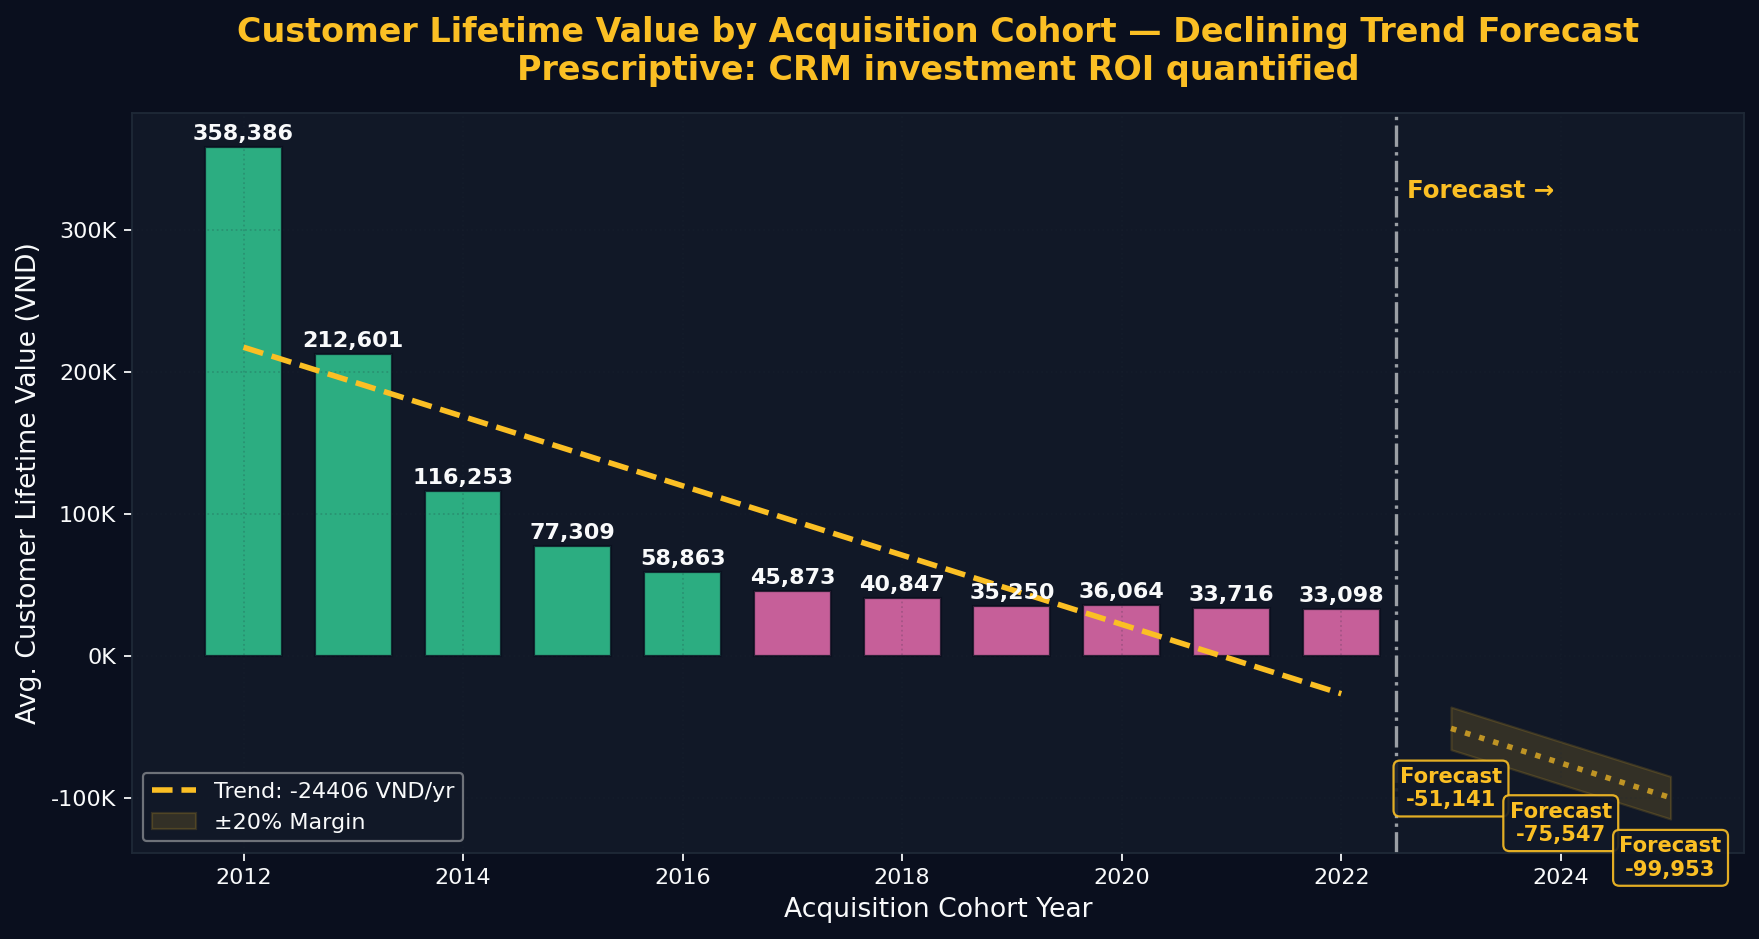
\includegraphics[width=\textwidth]{charts/1d_clv_decay_forecast.png}
    \caption{CLV decay: 358K $\to$ 33K VND. Slope: $-$24{,}406 VND/yr.}
    \label{fig:app1d}
  \end{subfigure}
  \caption{Insight 1 predictive signals.}
\end{figure}

%--- Insight 2 ---
\subsection{Insight 2: Promo Paradox}
\label{app:insight2}

\begin{figure}[htbp]
  \centering
  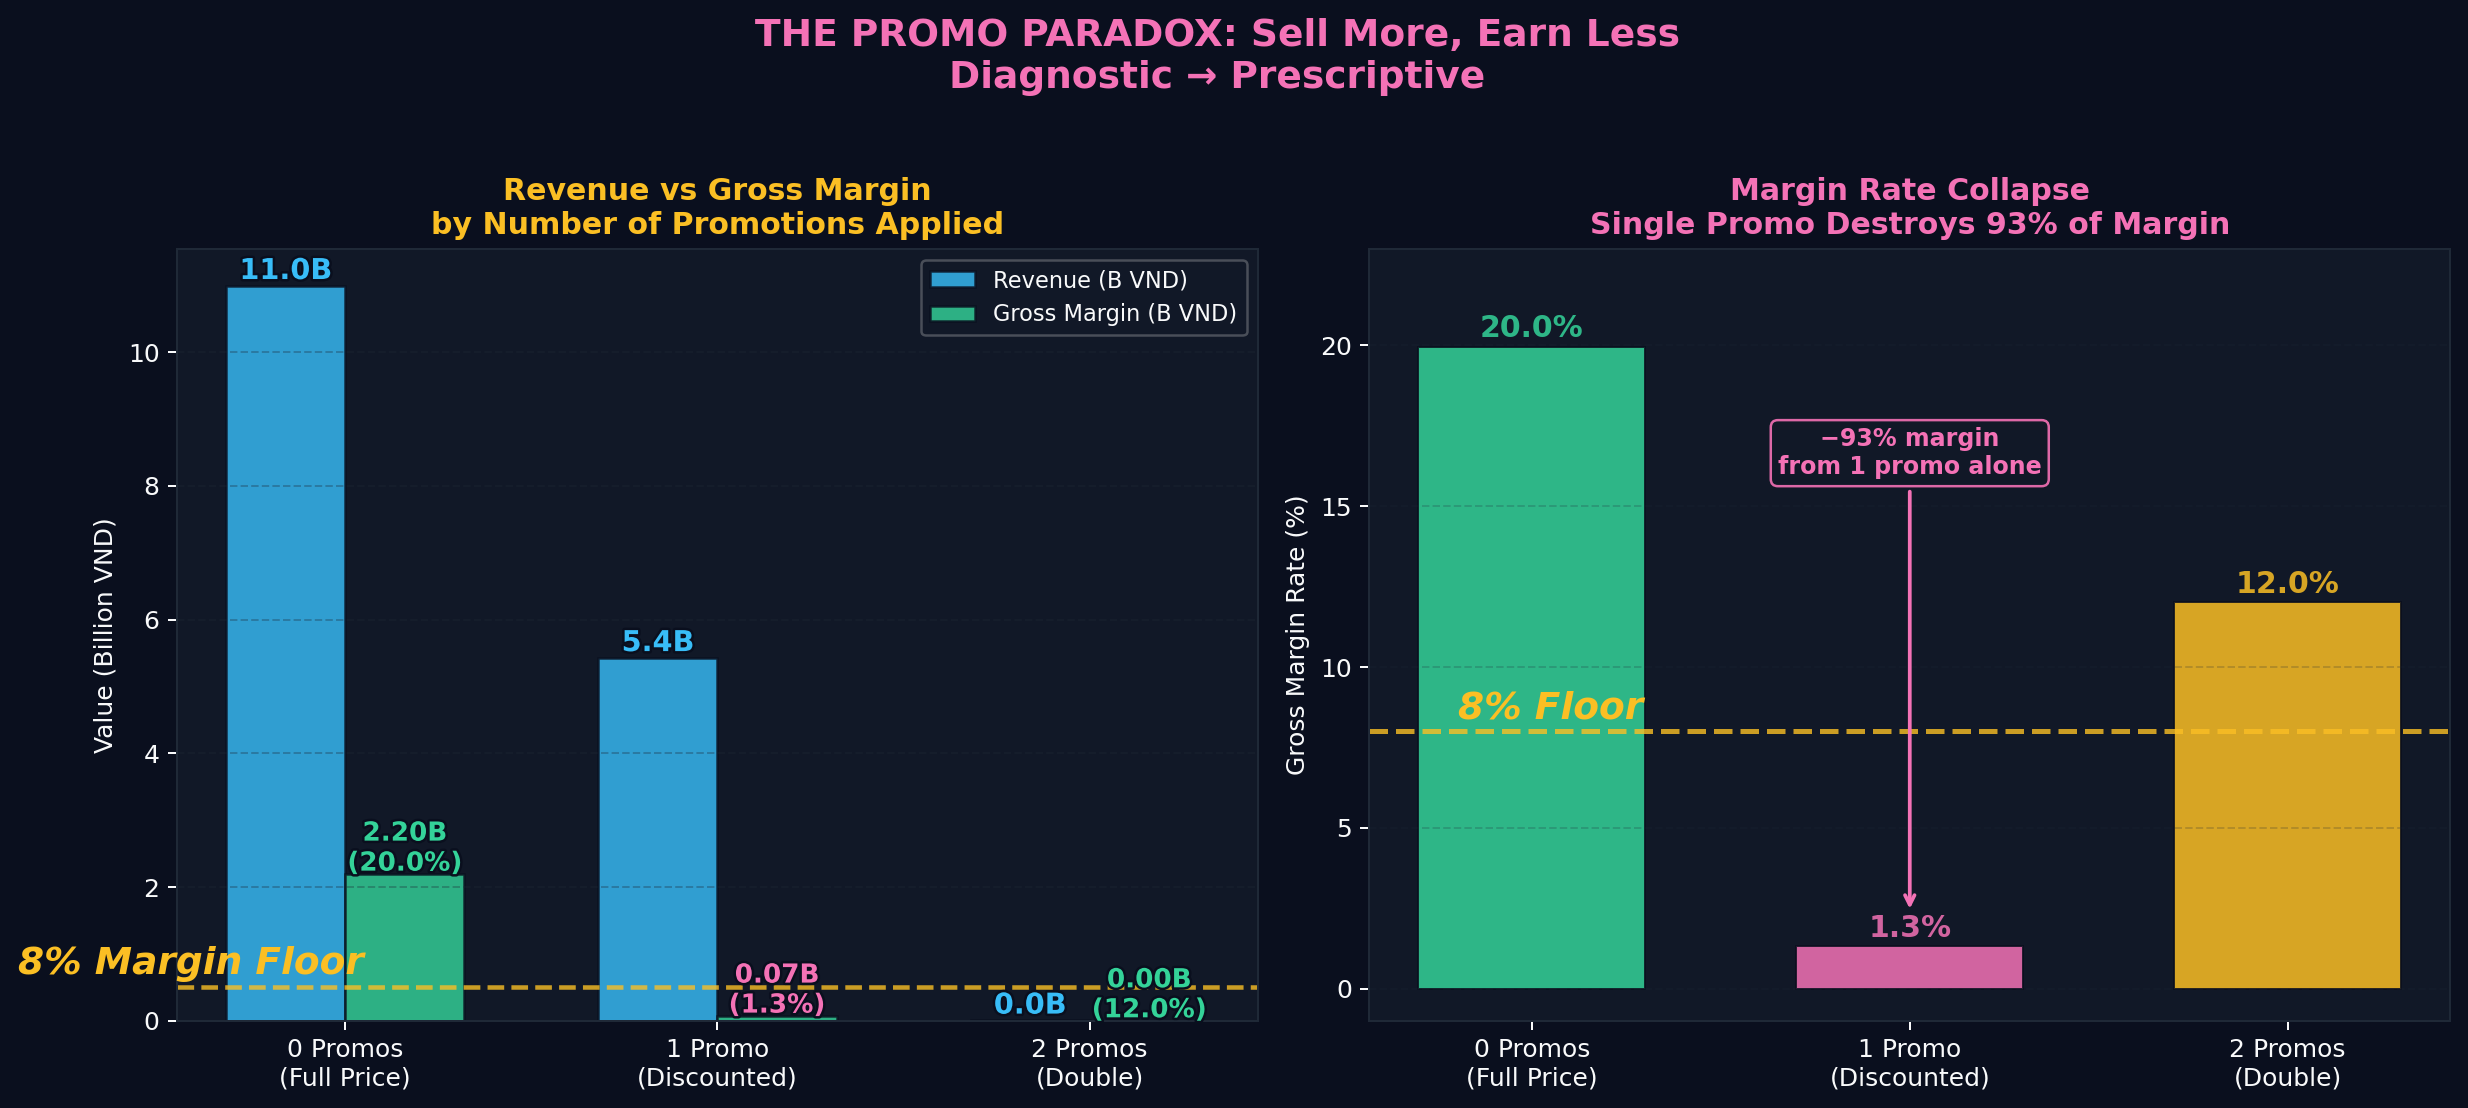
\includegraphics[width=\textwidth]{charts/2a_promo_margin_collapse.png}
  \caption{A single promotion cuts margin from 20.0\% to 1.3\%---93\% destruction.}
  \label{fig:app2a}
\end{figure}

\begin{figure}[htbp]
  \centering
  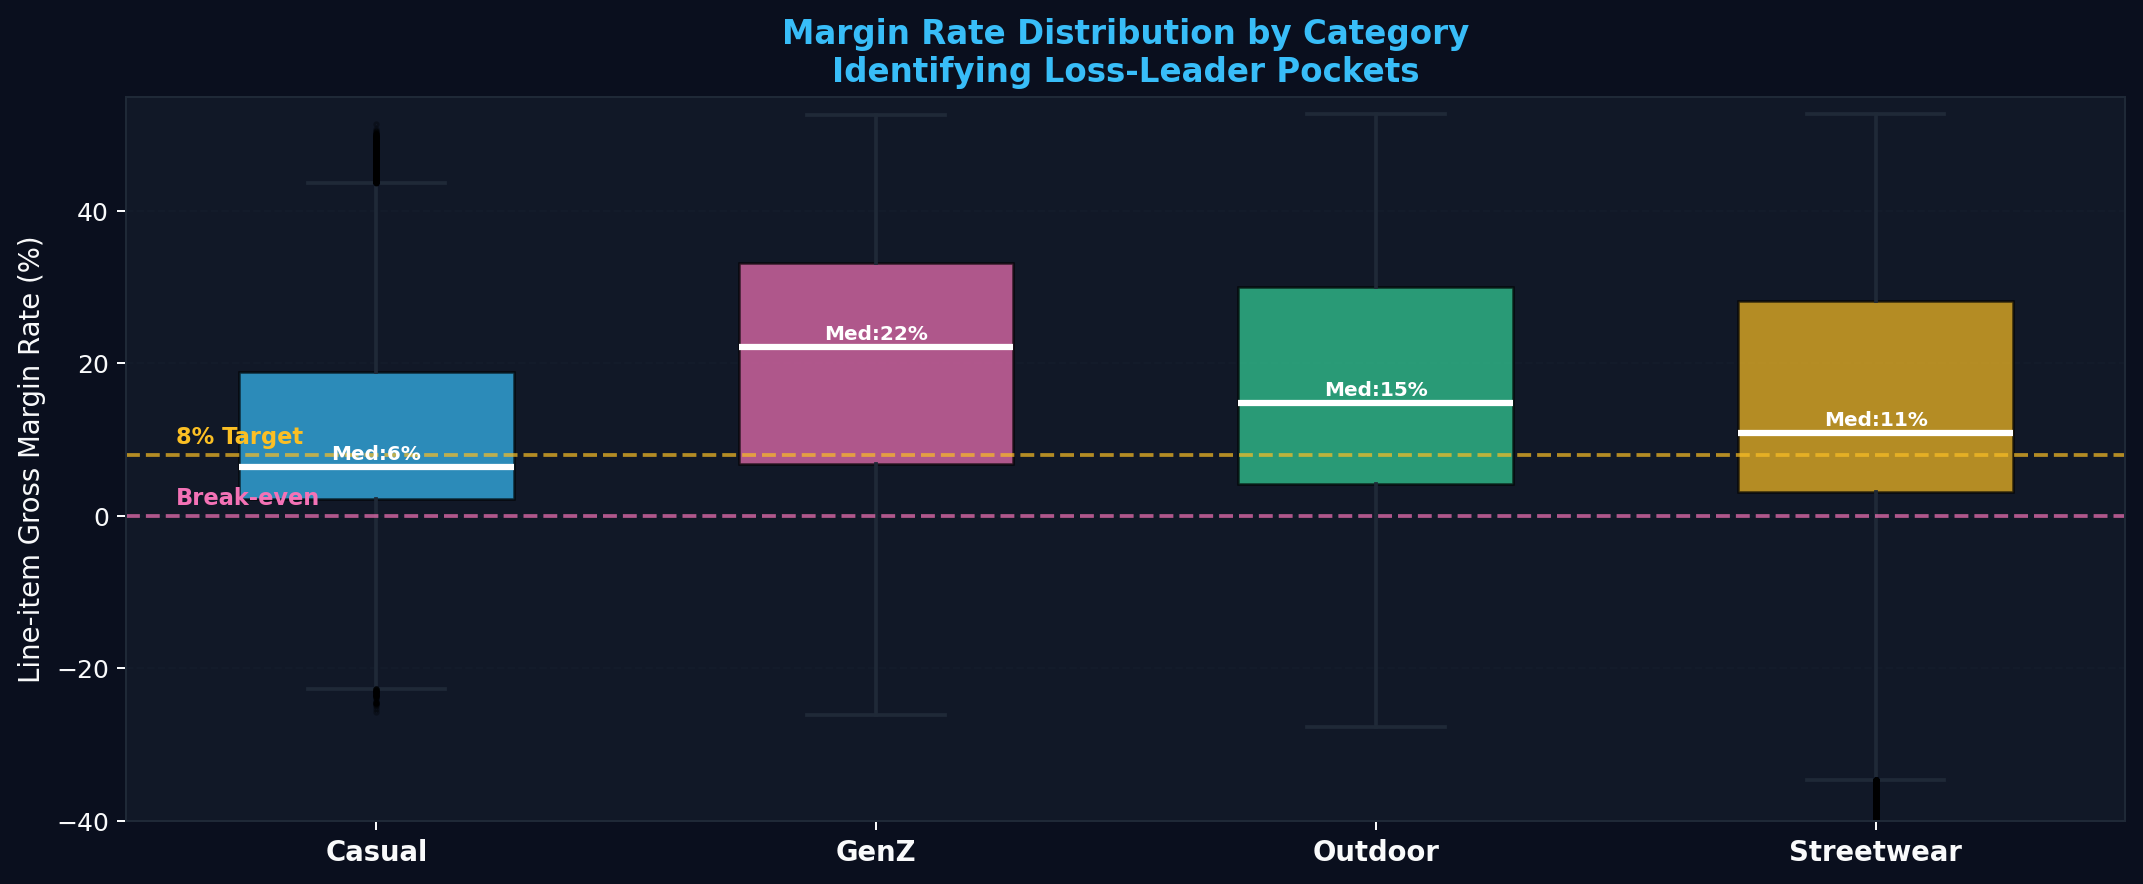
\includegraphics[width=\textwidth]{charts/2b_margin_by_category_boxplot.png}
  \caption{Margin distribution by category. Casual median: 6\%. GenZ median: 22\%.}
  \label{fig:app2b}
\end{figure}

\begin{figure}[htbp]
  \centering
  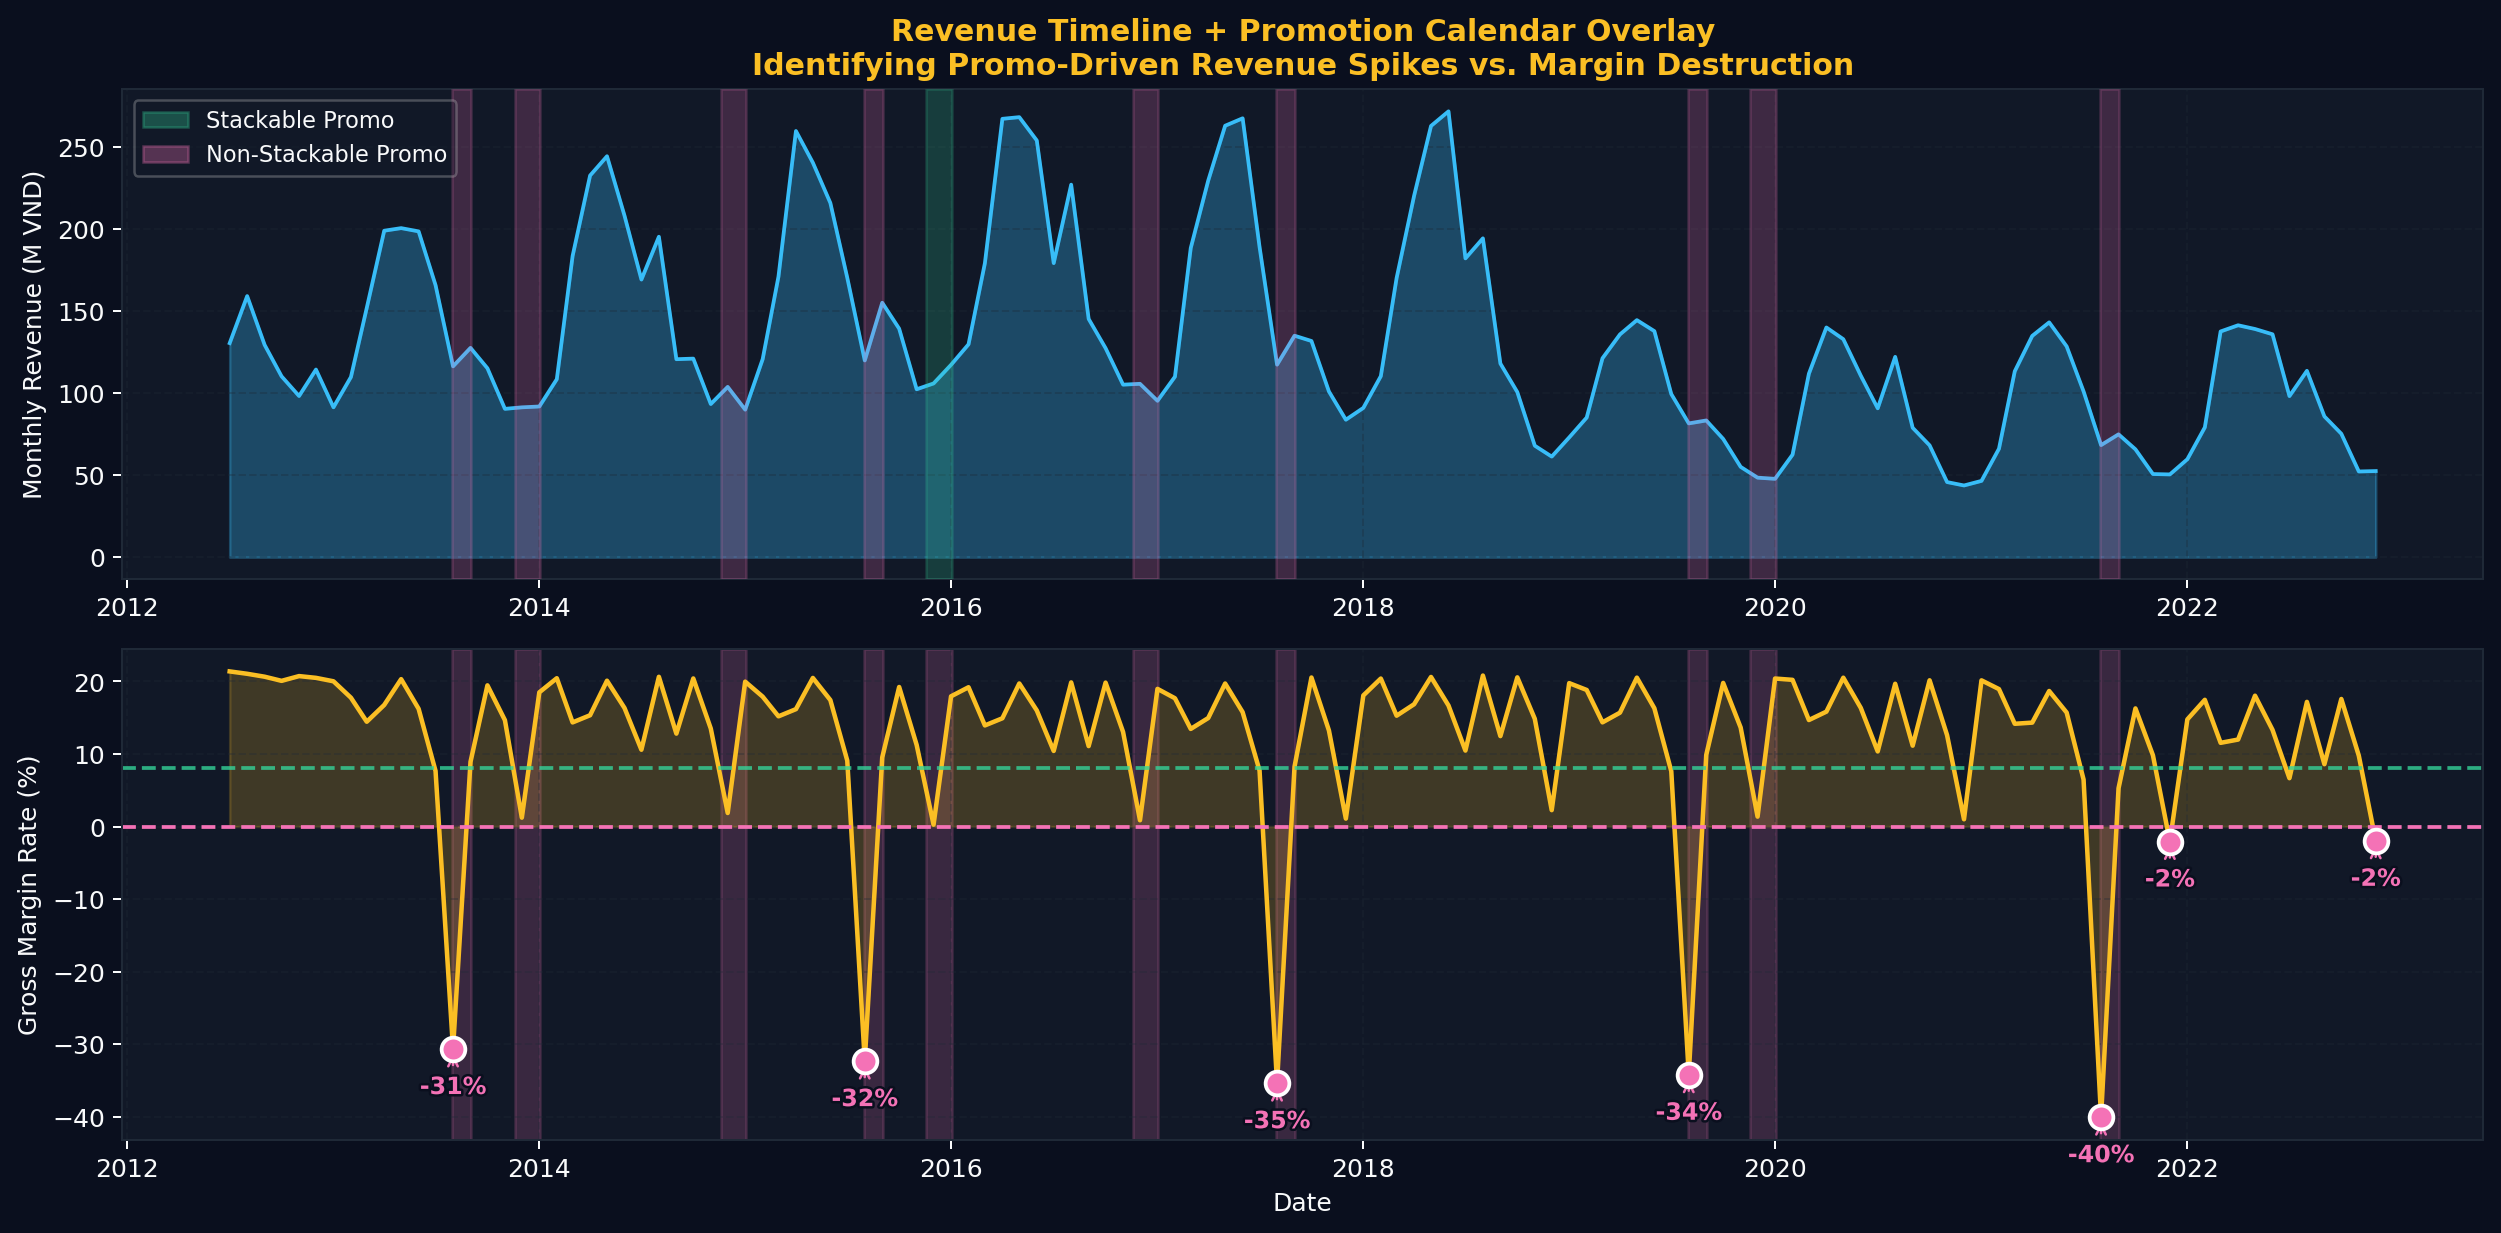
\includegraphics[width=\textwidth]{charts/2c_promo_timeline.png}
  \caption{Revenue timeline with promotion calendar. Worst month: $-$40\% gross margin.}
  \label{fig:app2c}
\end{figure}

\begin{figure}[htbp]
  \centering
  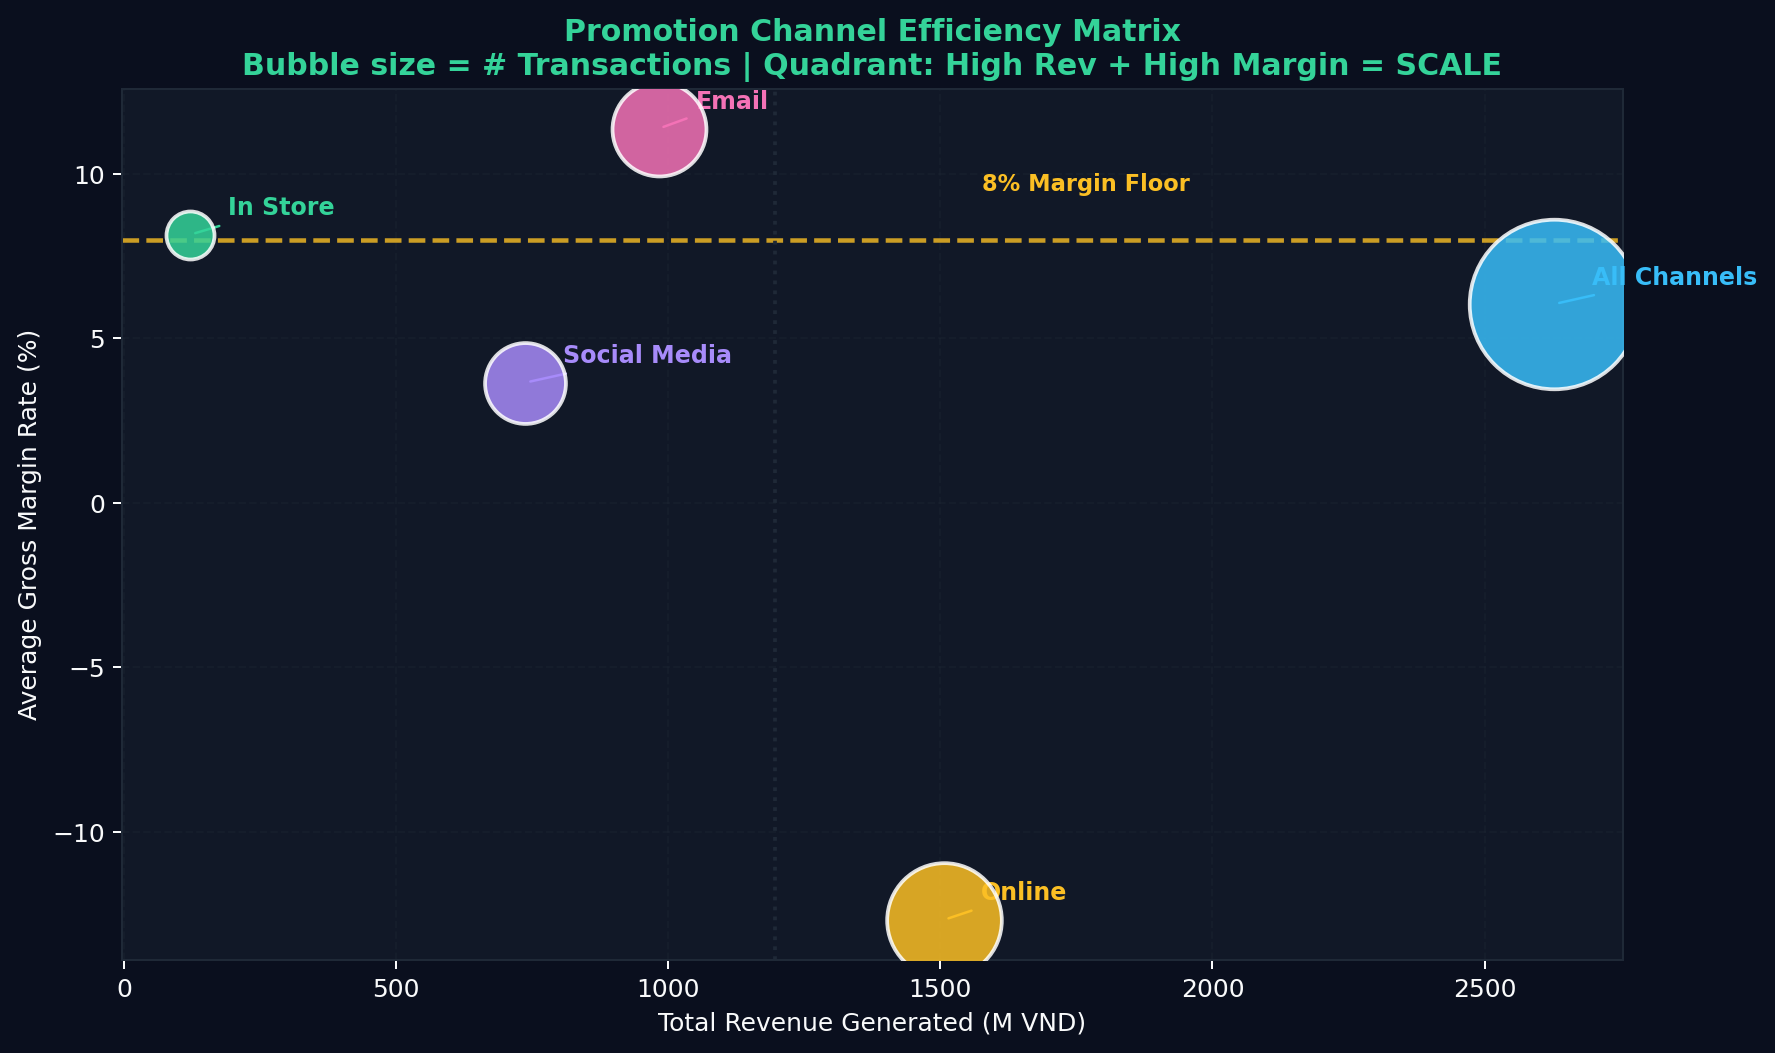
\includegraphics[width=0.65\textwidth]{charts/2d_promo_channel_efficiency.png}
  \caption{Channel efficiency: \texttt{all\_channels} = most revenue, lowest margin.}
  \label{fig:app2d}
\end{figure}

%--- Insight 3 ---
\subsection{Insight 3: Wrong-Size Tax}
\label{app:insight3}

\begin{figure}[htbp]
  \centering
  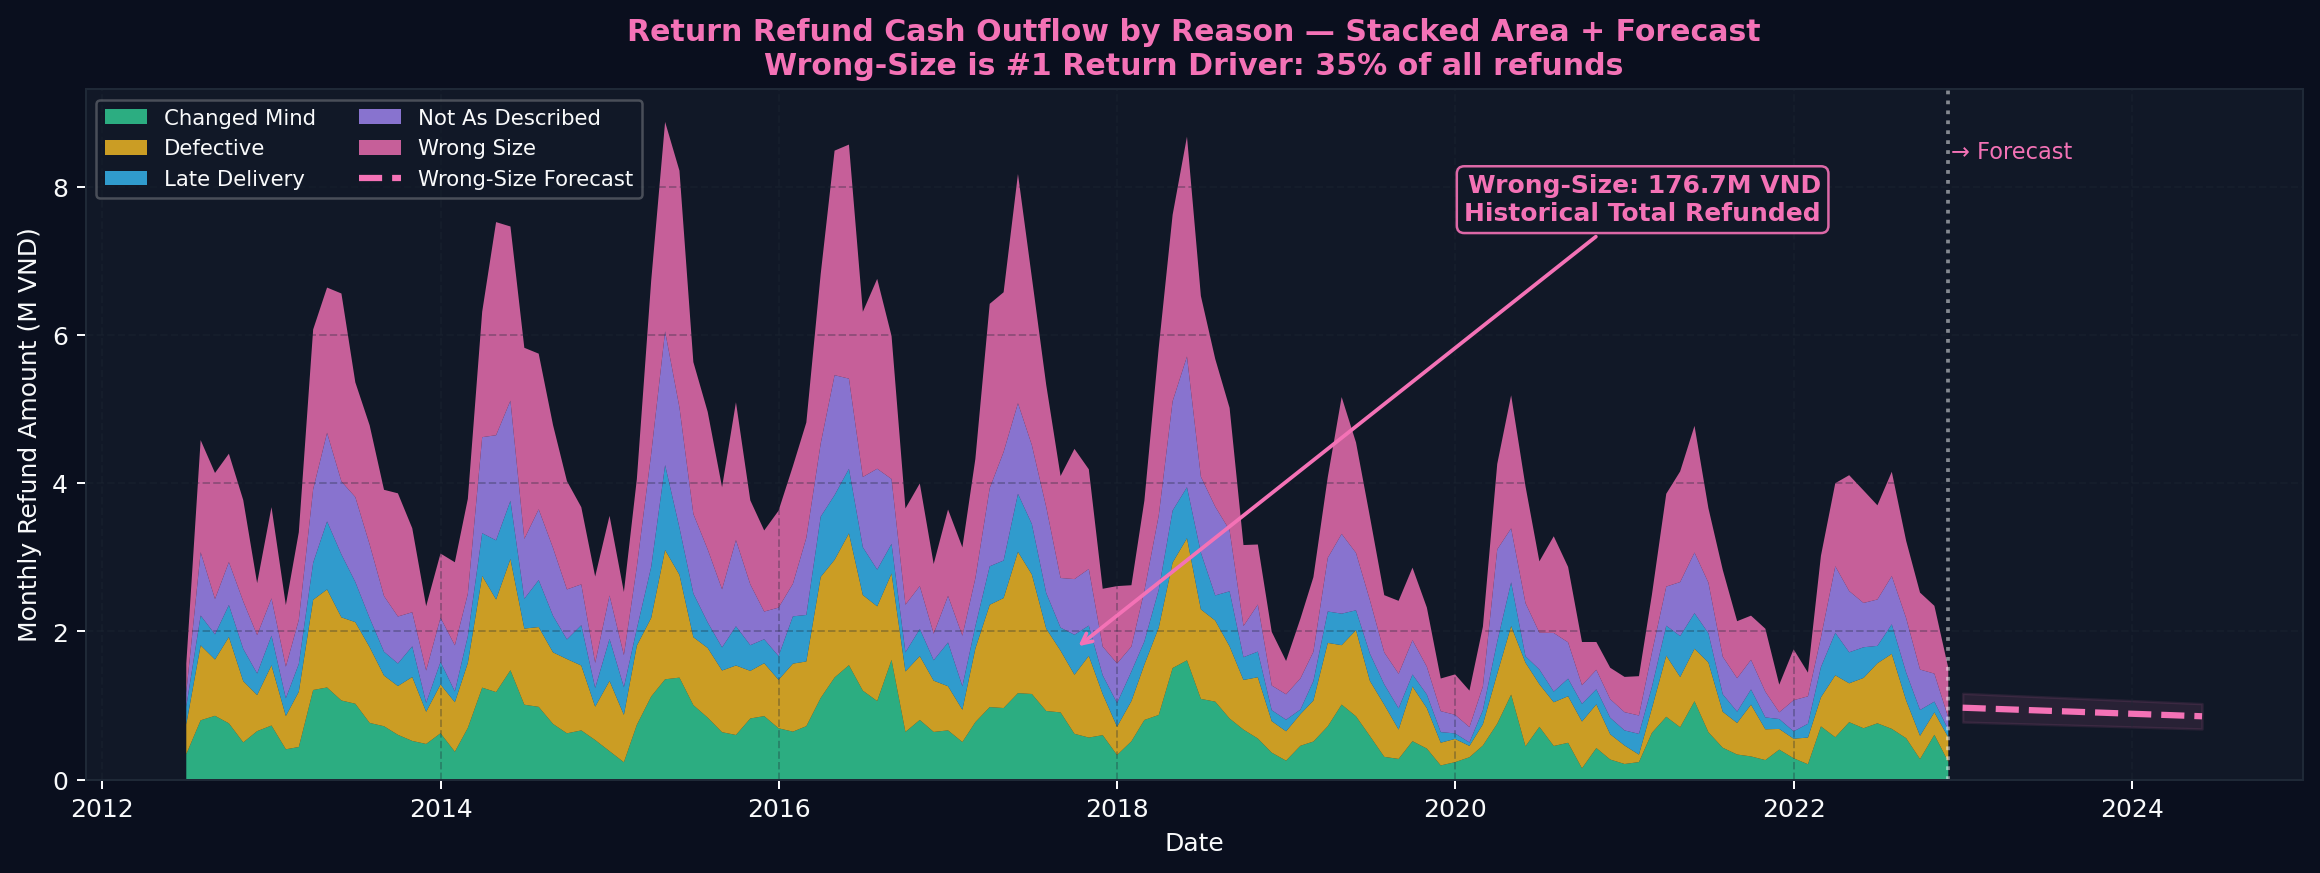
\includegraphics[width=\textwidth]{charts/3a_returns_stacked_forecast.png}
  \caption{Monthly refund outflow by return reason with wrong-size forecast.}
  \label{fig:app3a}
\end{figure}

\begin{figure}[htbp]
  \centering
  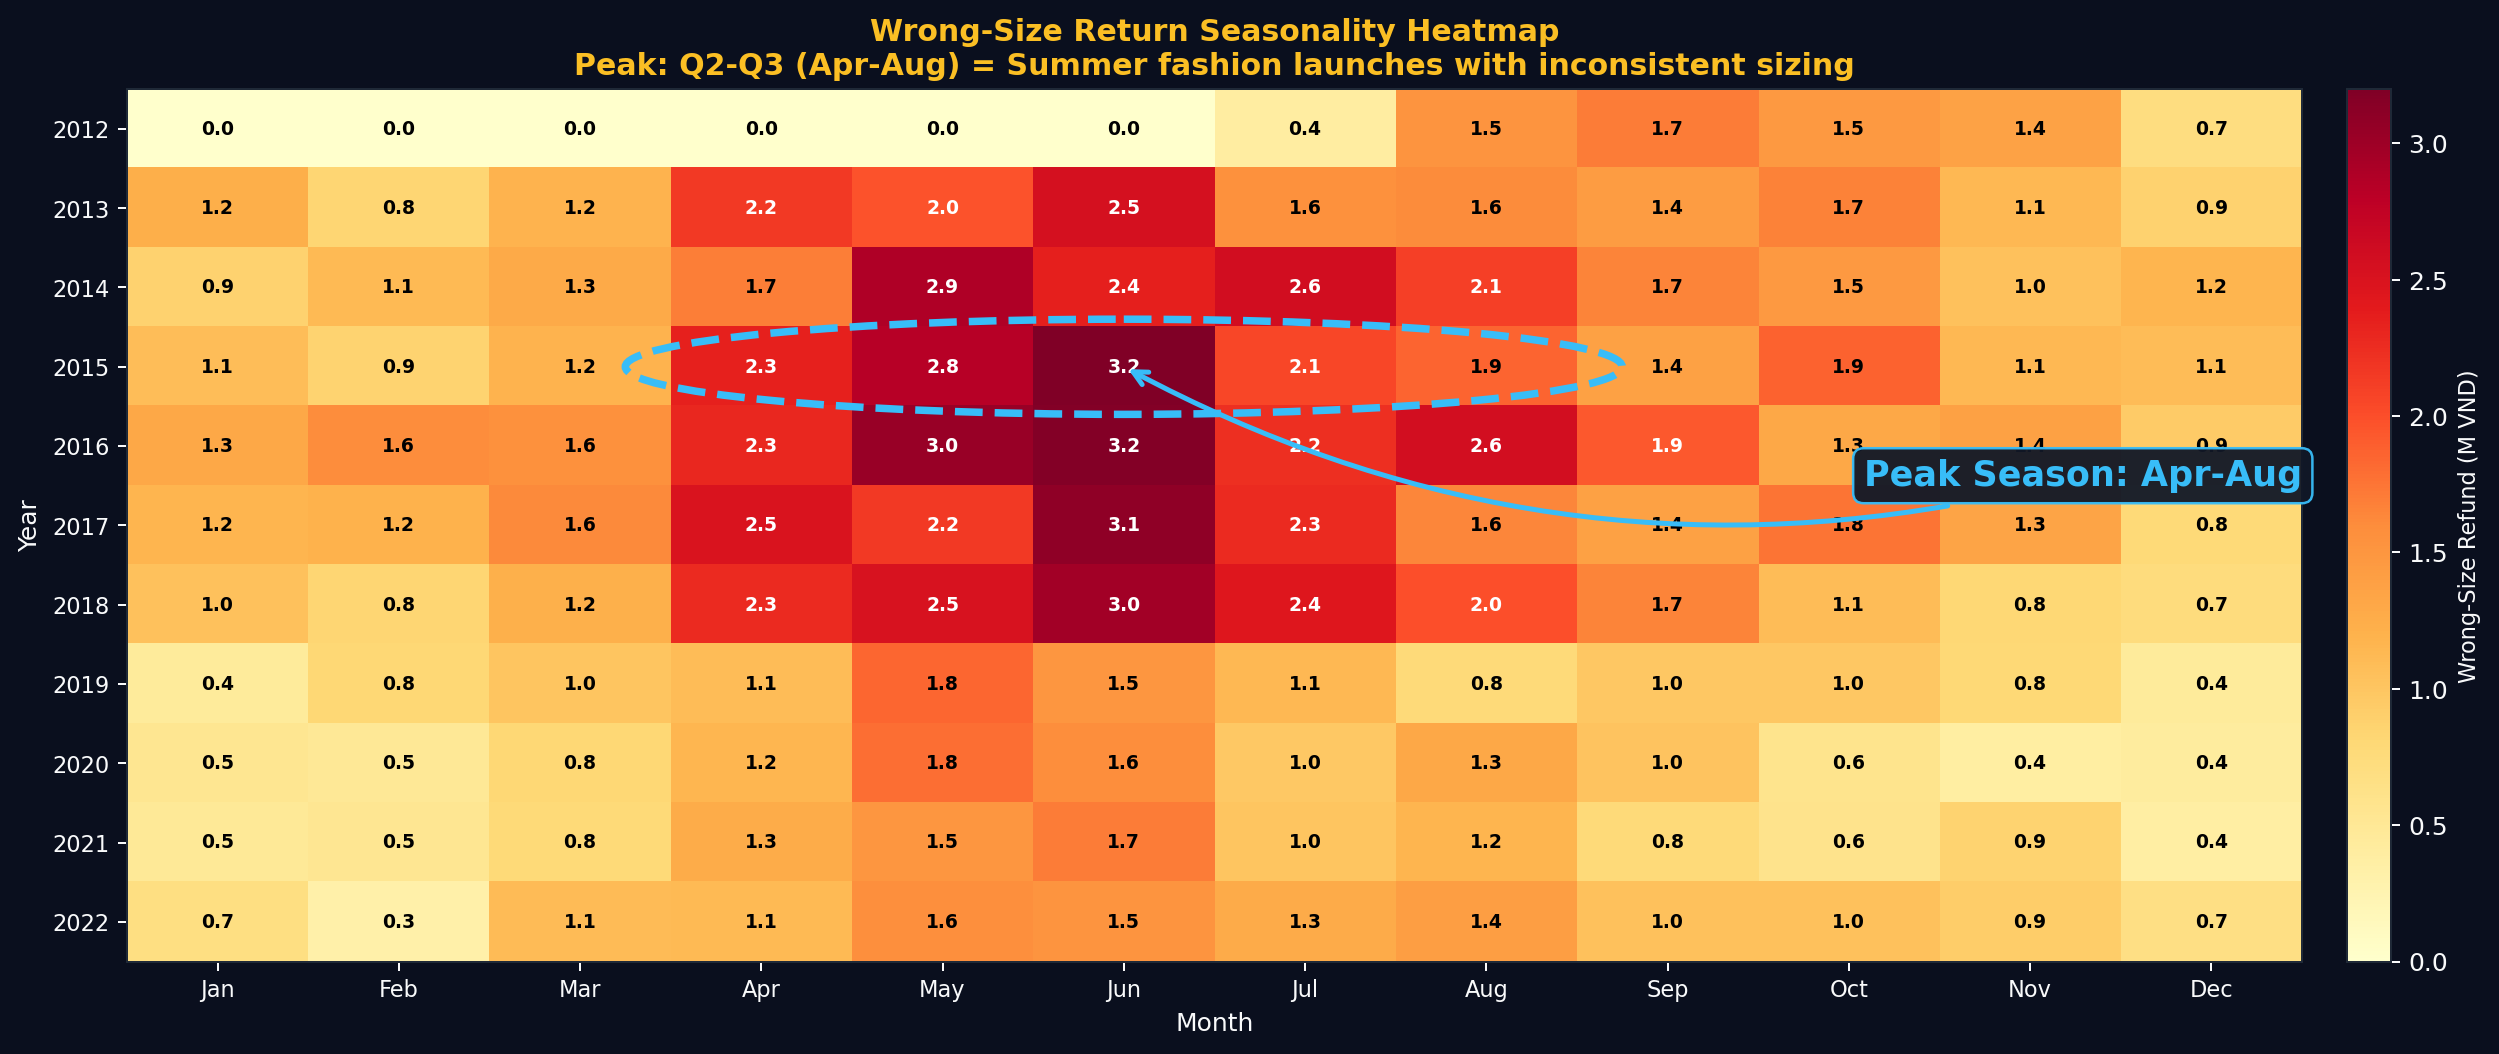
\includegraphics[width=\textwidth]{charts/3d_wrongsize_seasonal_heatmap.png}
  \caption{Wrong-size seasonality: Apr--Aug corridor consistently peaks.}
  \label{fig:app3d}
\end{figure}

%--- Insight 4 ---
\subsection{Insight 4: Stockout Bleeding}
\label{app:insight4}

\begin{figure}[htbp]
  \centering
  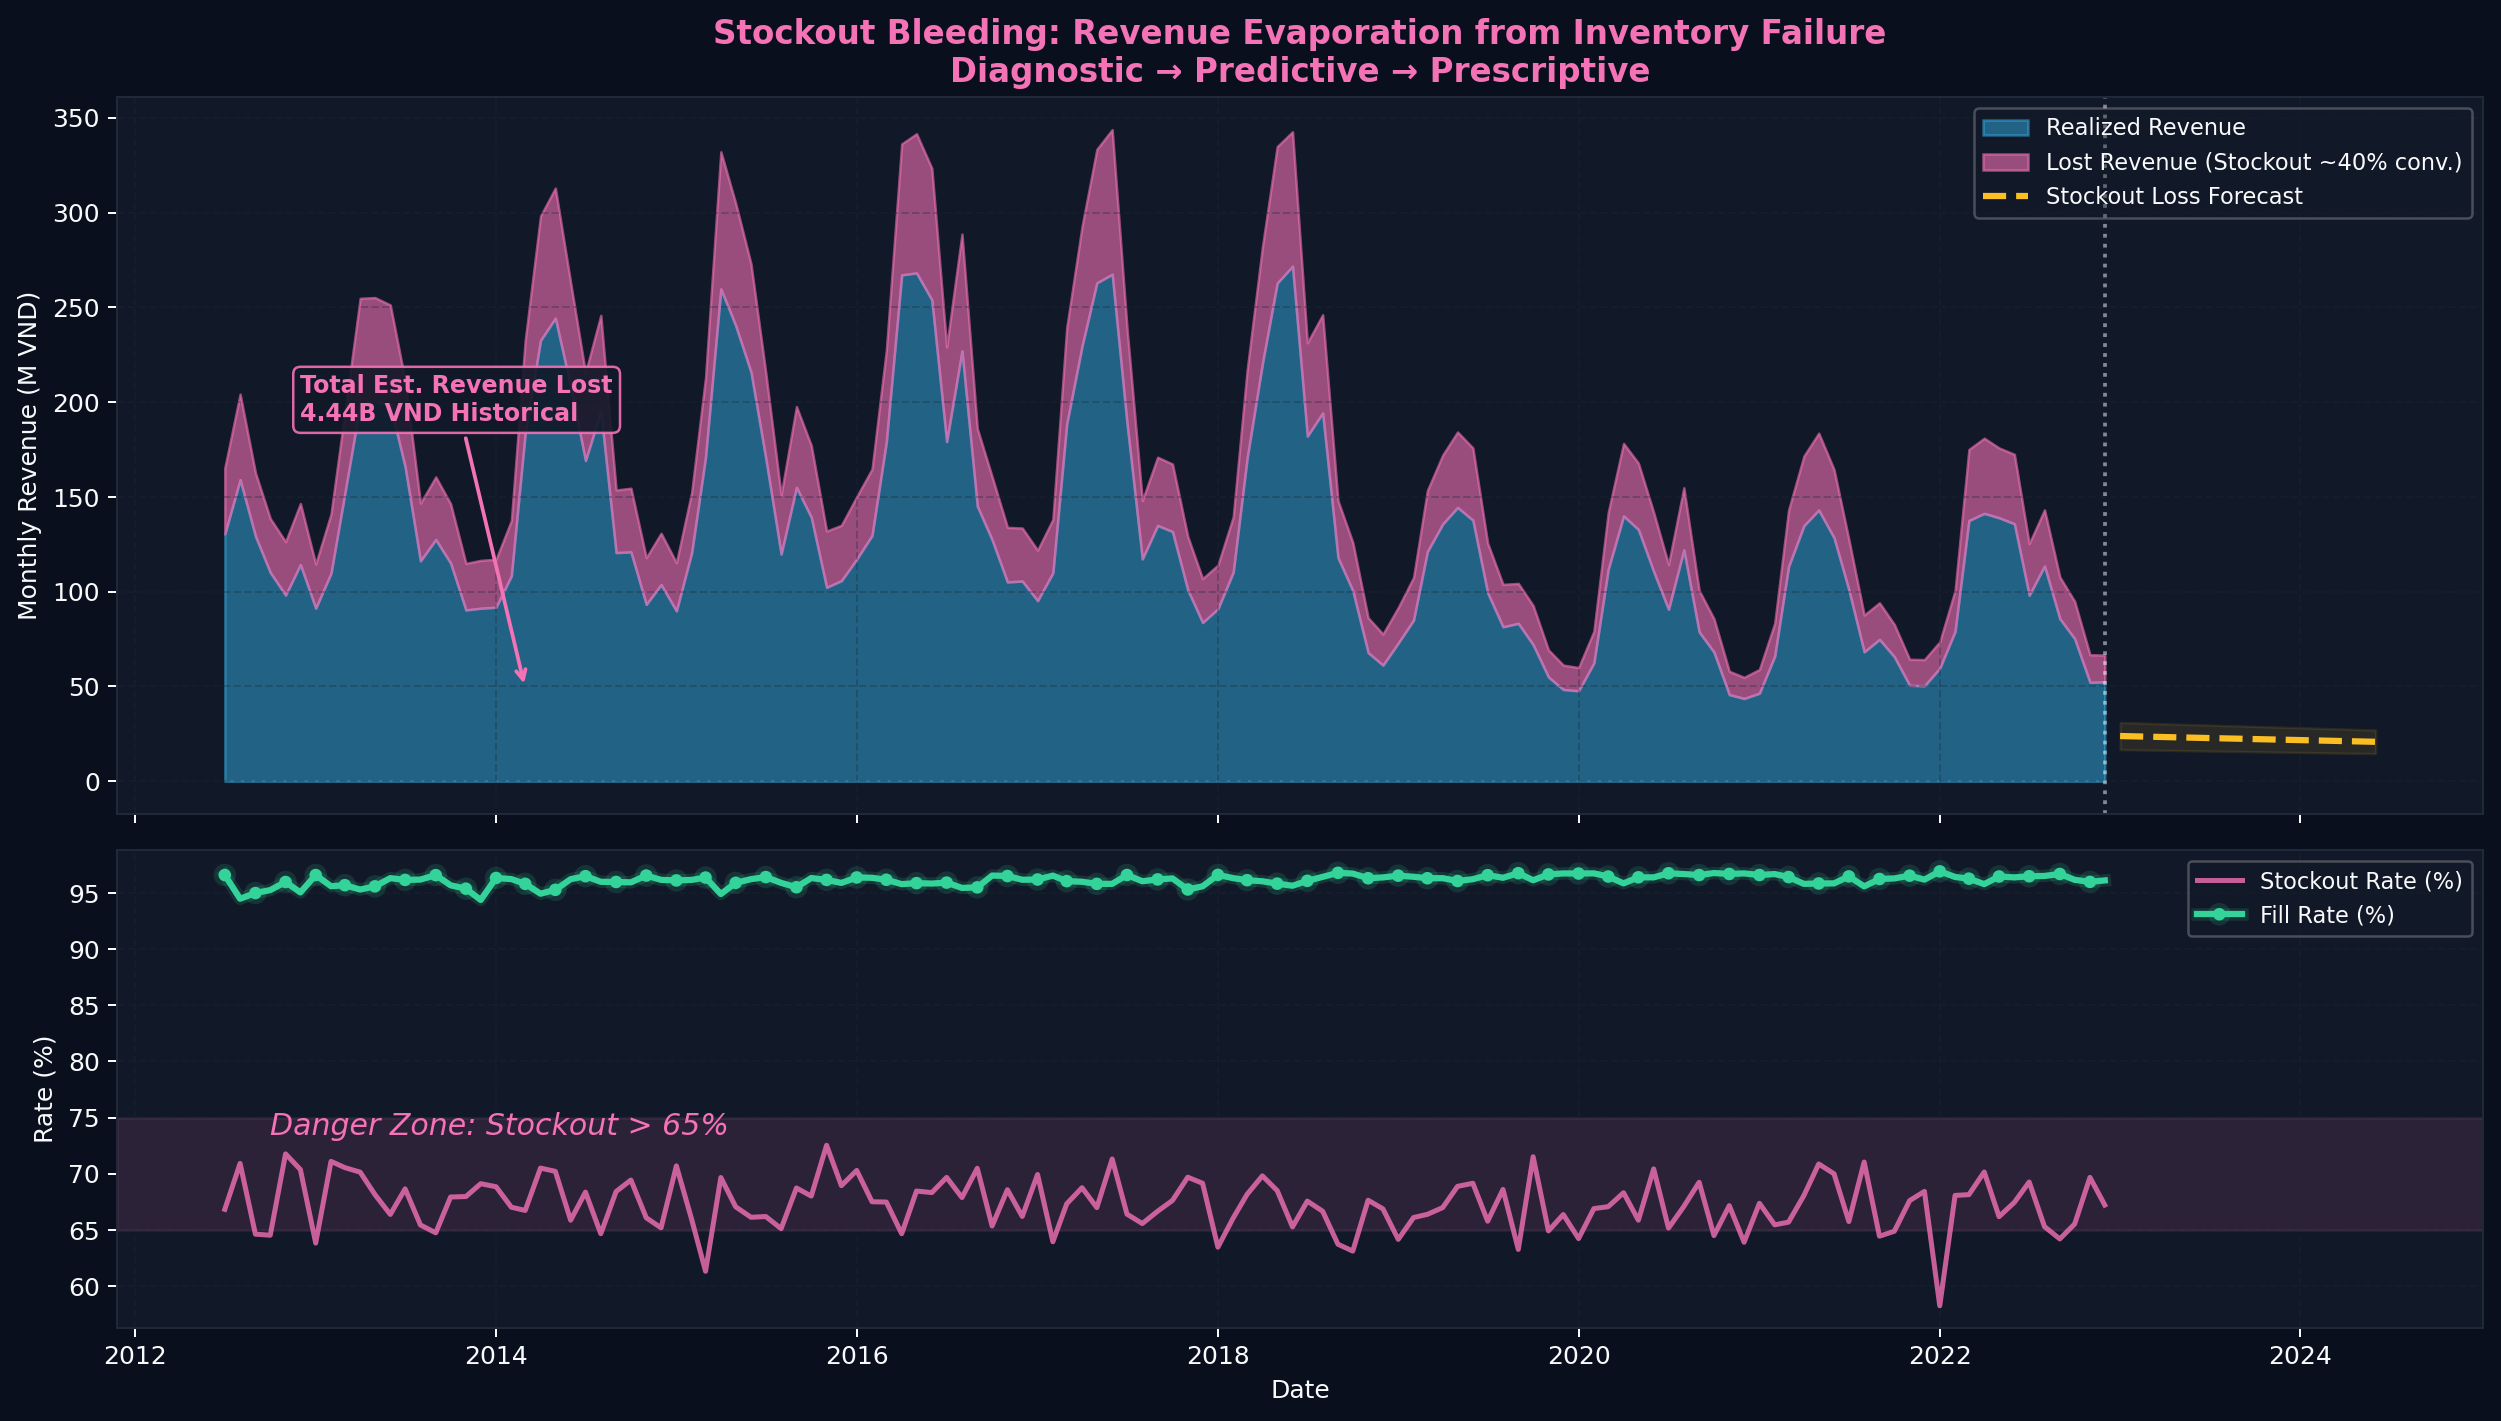
\includegraphics[width=\textwidth]{charts/4a_stockout_bleeding.png}
  \caption{Stockout revenue evaporation. Top: realized vs.\ estimated lost revenue (4.44B VND). Bottom: stockout rate (67\%) vs.\ fill rate (96\%).}
  \label{fig:app4a}
\end{figure}

\begin{figure}[htbp]
  \centering
  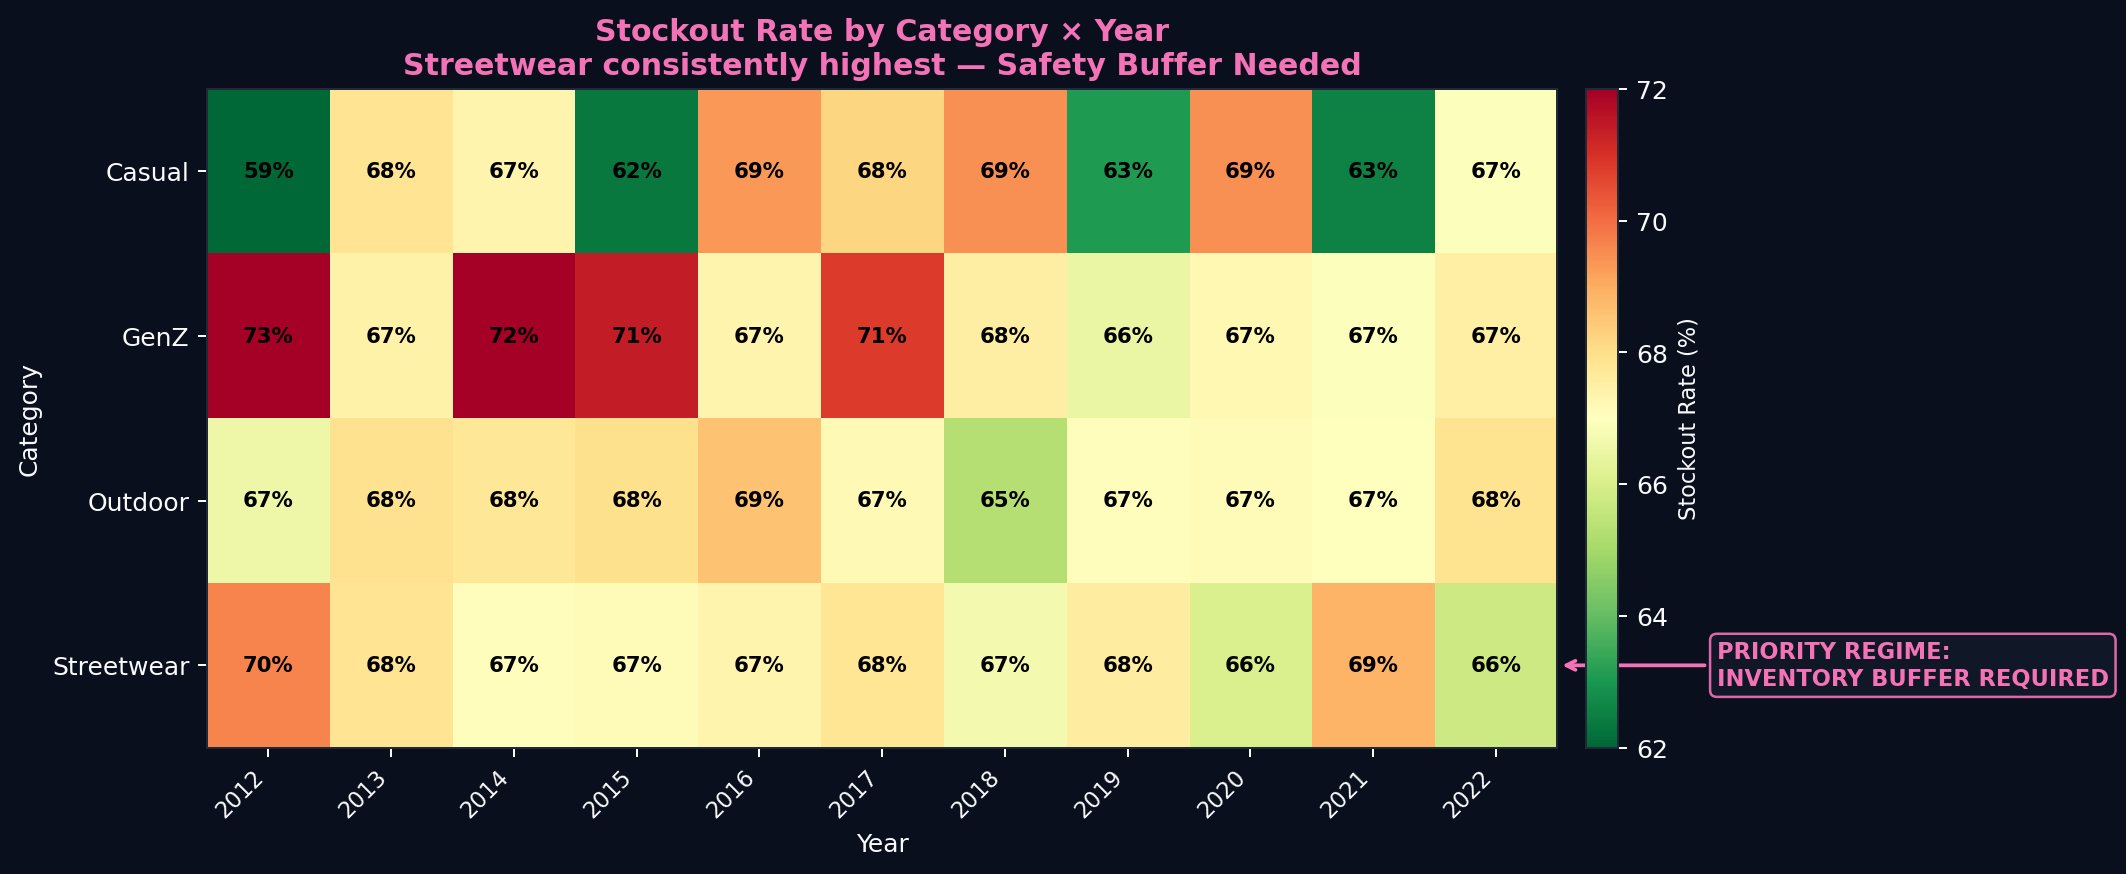
\includegraphics[width=\textwidth]{charts/4b_stockout_by_category_heatmap.png}
  \caption{Stockout rate by category $\times$ year. GenZ: 73\% peak. Streetwear: 66--70\%.}
  \label{fig:app4b}
\end{figure}

\begin{figure}[htbp]
  \centering
  \begin{subfigure}[t]{0.48\textwidth}
    \centering
    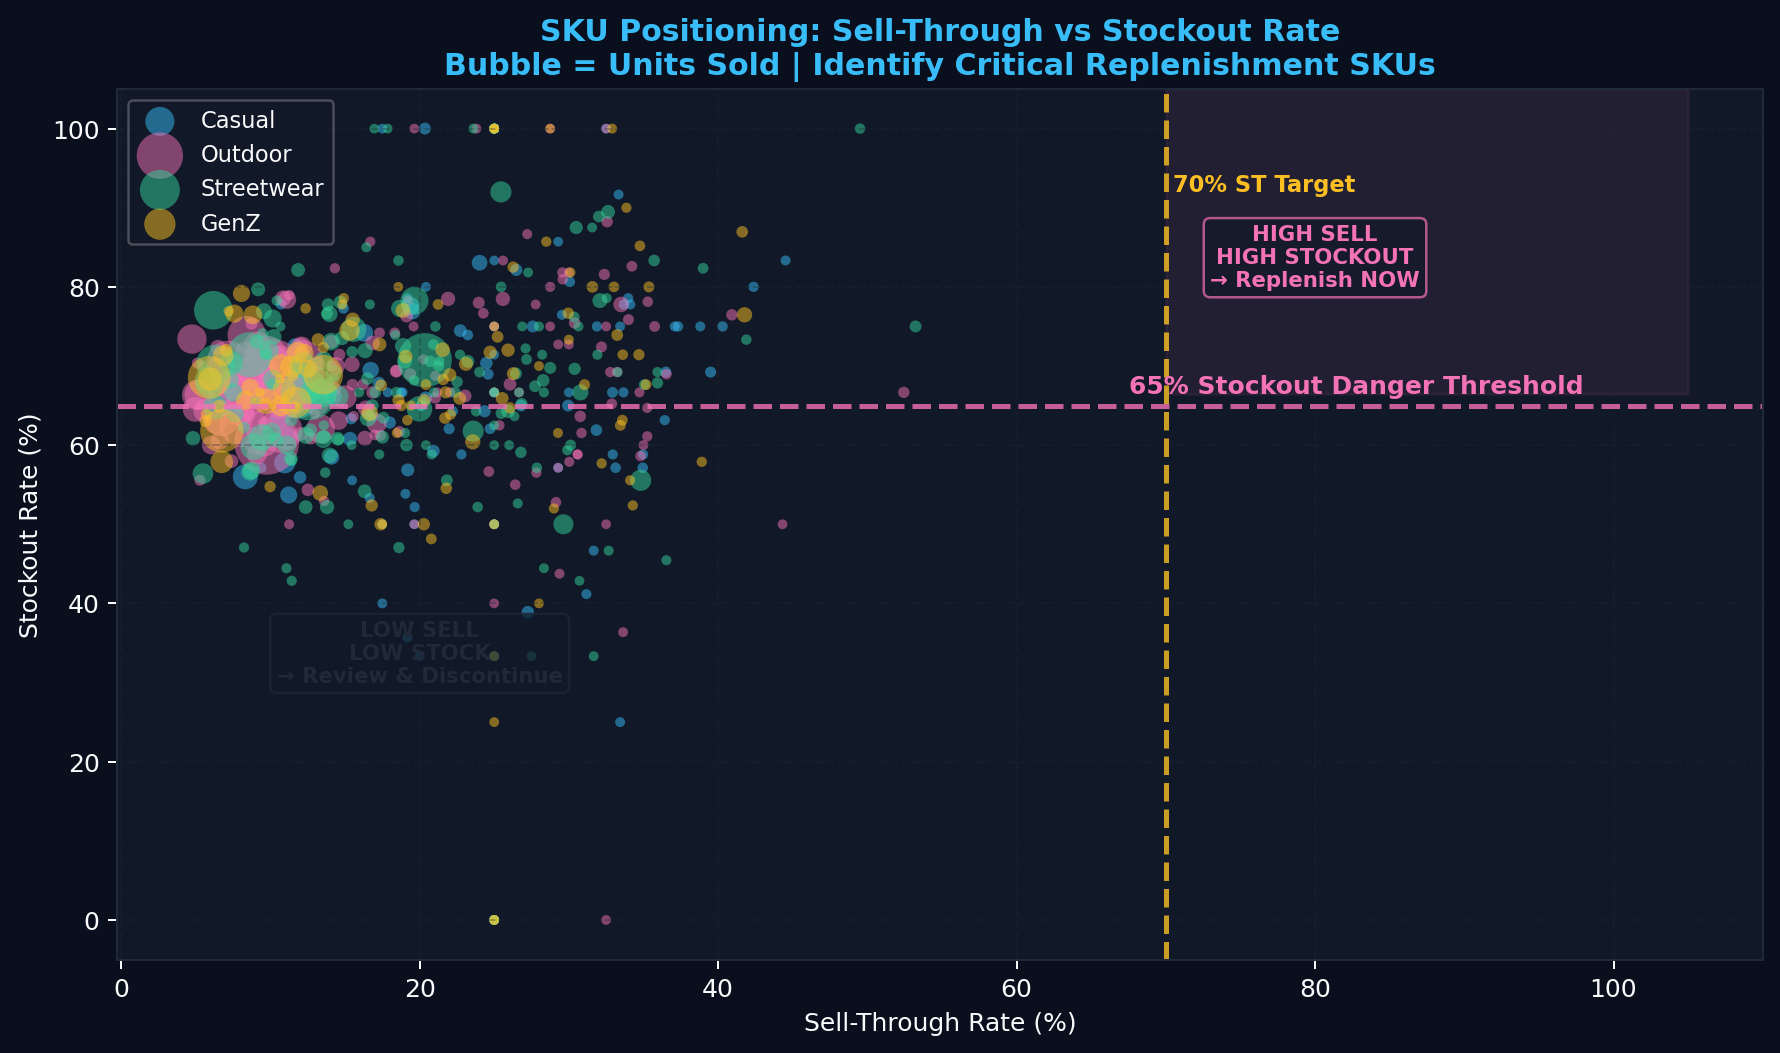
\includegraphics[width=\textwidth]{charts/4c_sellthrough_vs_stockout.png}
    \caption{SKU positioning: high sell-through + high stockout = urgent.}
    \label{fig:app4c}
  \end{subfigure}\hfill
  \begin{subfigure}[t]{0.48\textwidth}
    \centering
    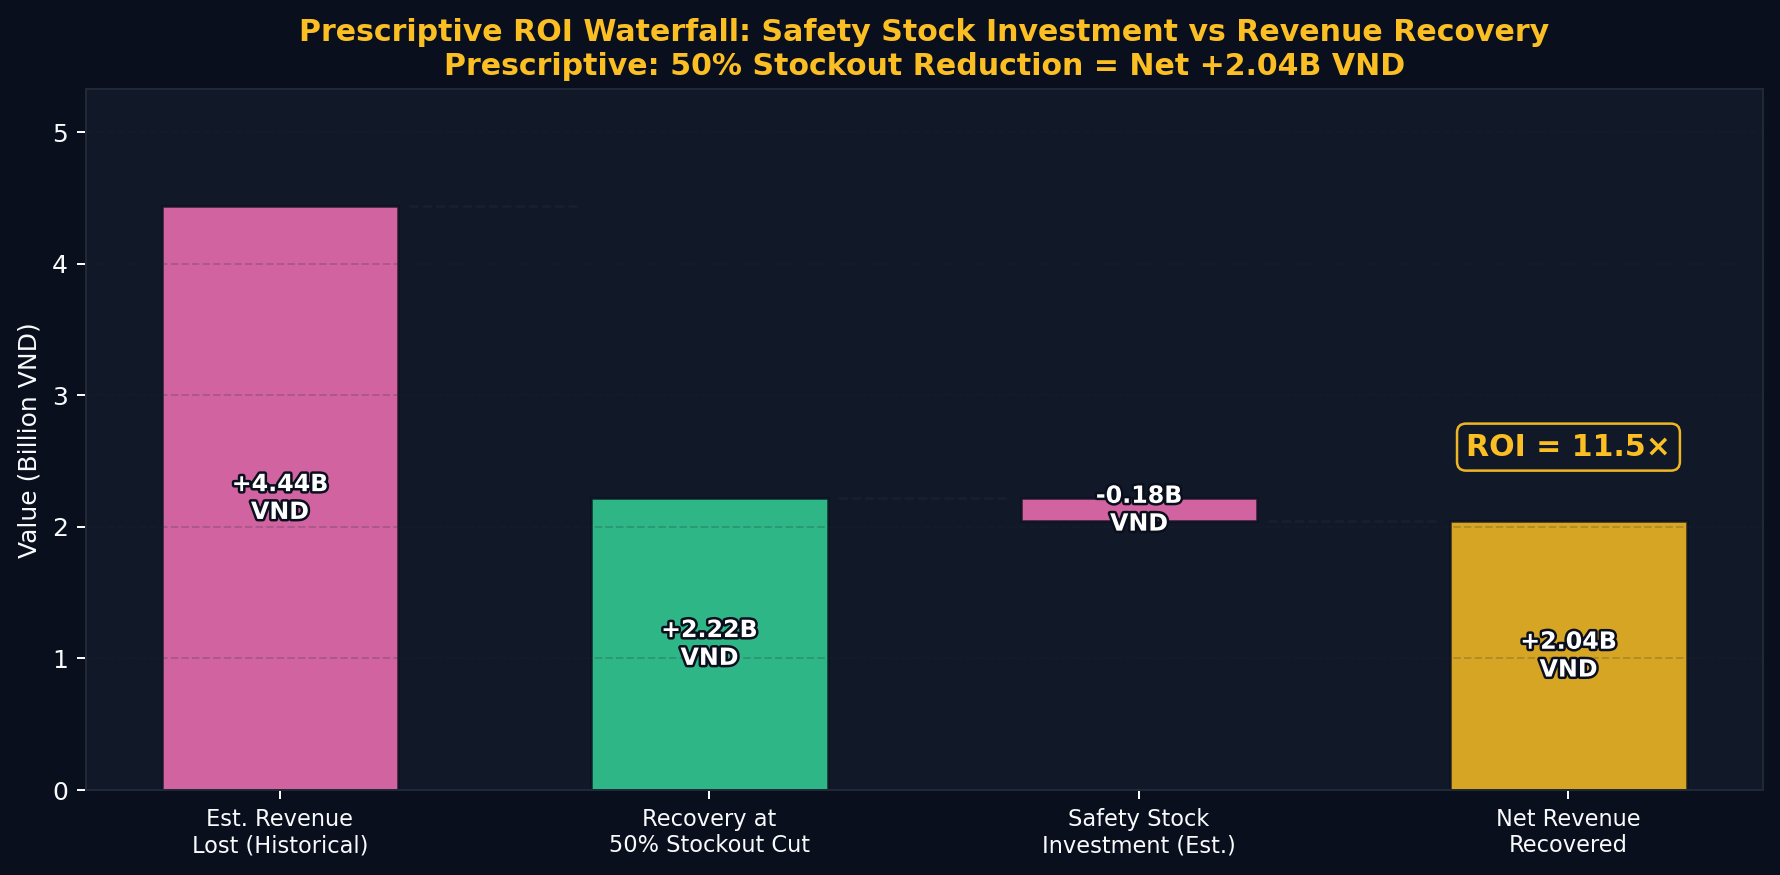
\includegraphics[width=\textwidth]{charts/4d_stockout_roi_waterfall.png}
    \caption{ROI waterfall: net +2.04B VND (11.5$\times$).}
    \label{fig:app4d}
  \end{subfigure}
  \caption{Insight 4 diagnostic and prescriptive exhibits.}
\end{figure}

%--- Insight 5 ---
\subsection{Insight 5: Traffic Quality}
\label{app:insight5}

\begin{figure}[htbp]
  \centering
  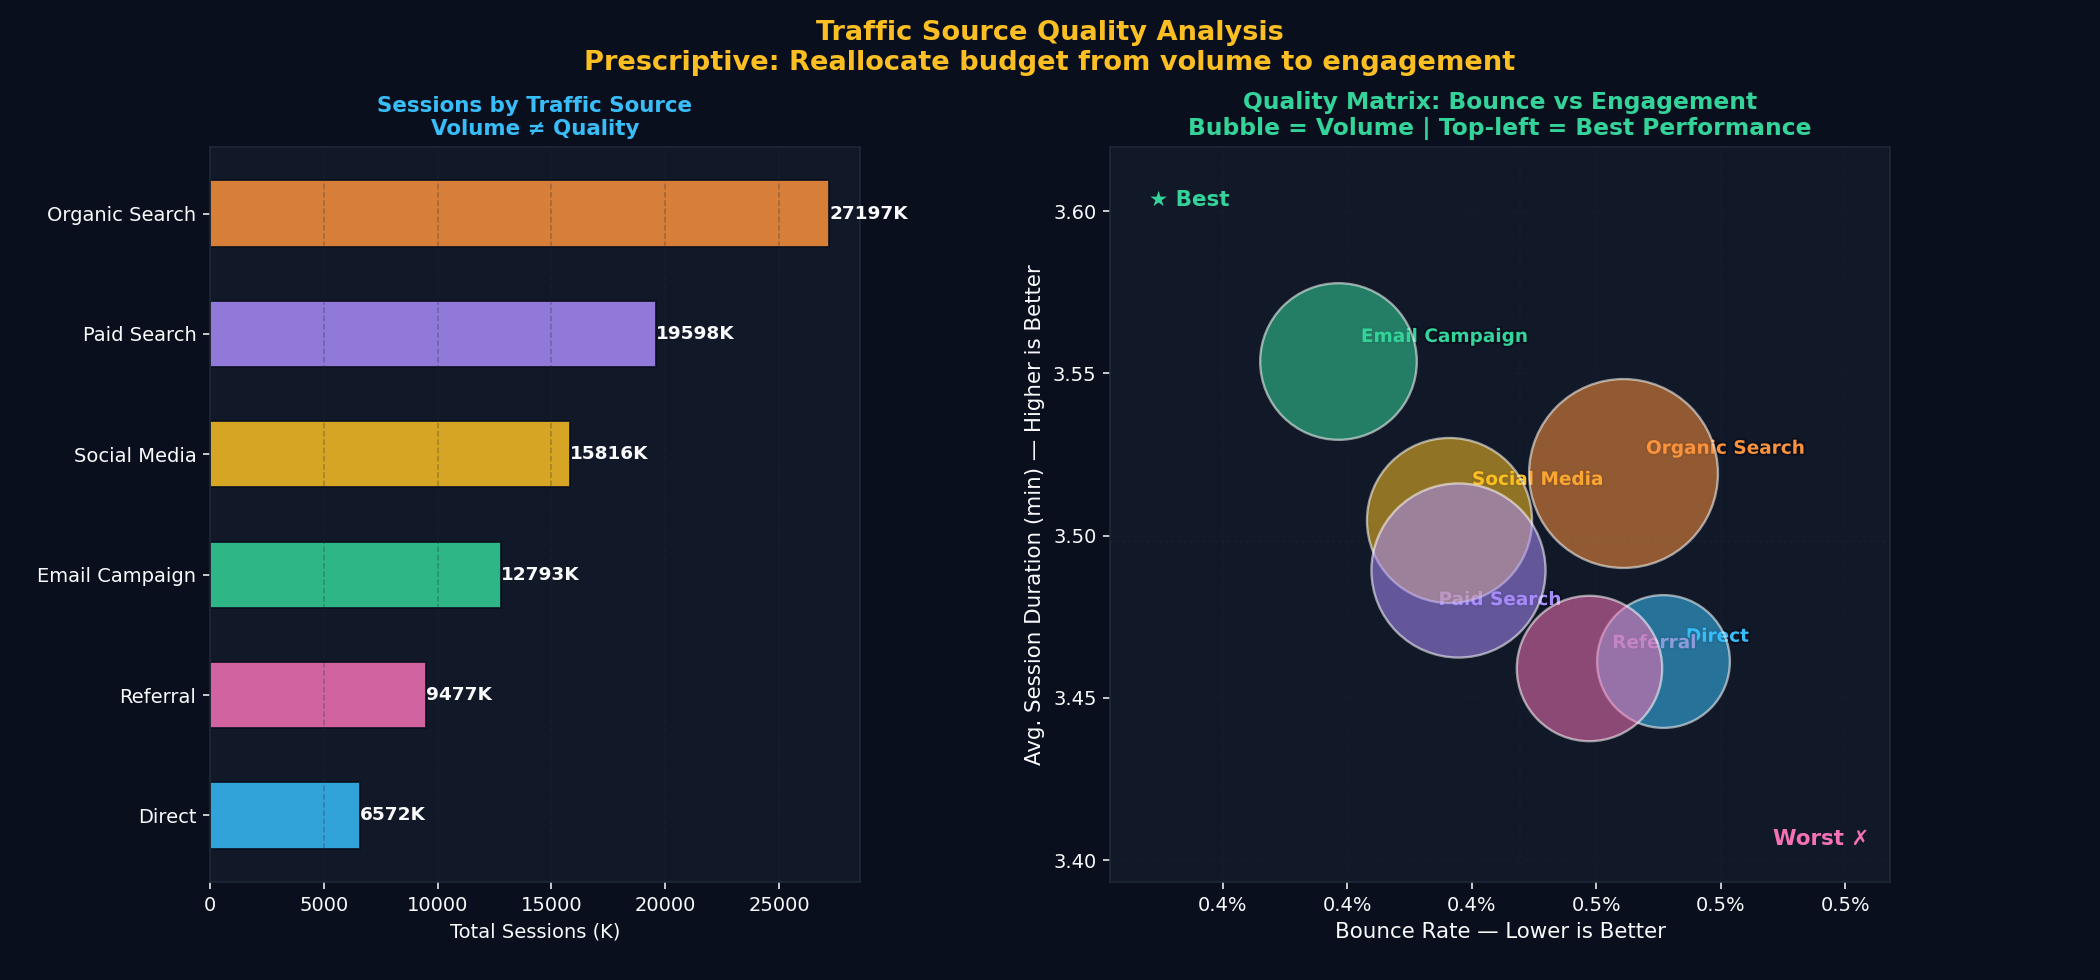
\includegraphics[width=\textwidth]{charts/5a_traffic_quality_matrix.png}
  \caption{Traffic source quality: email = lowest bounce, highest duration.}
  \label{fig:app5a}
\end{figure}

\begin{figure}[htbp]
  \centering
  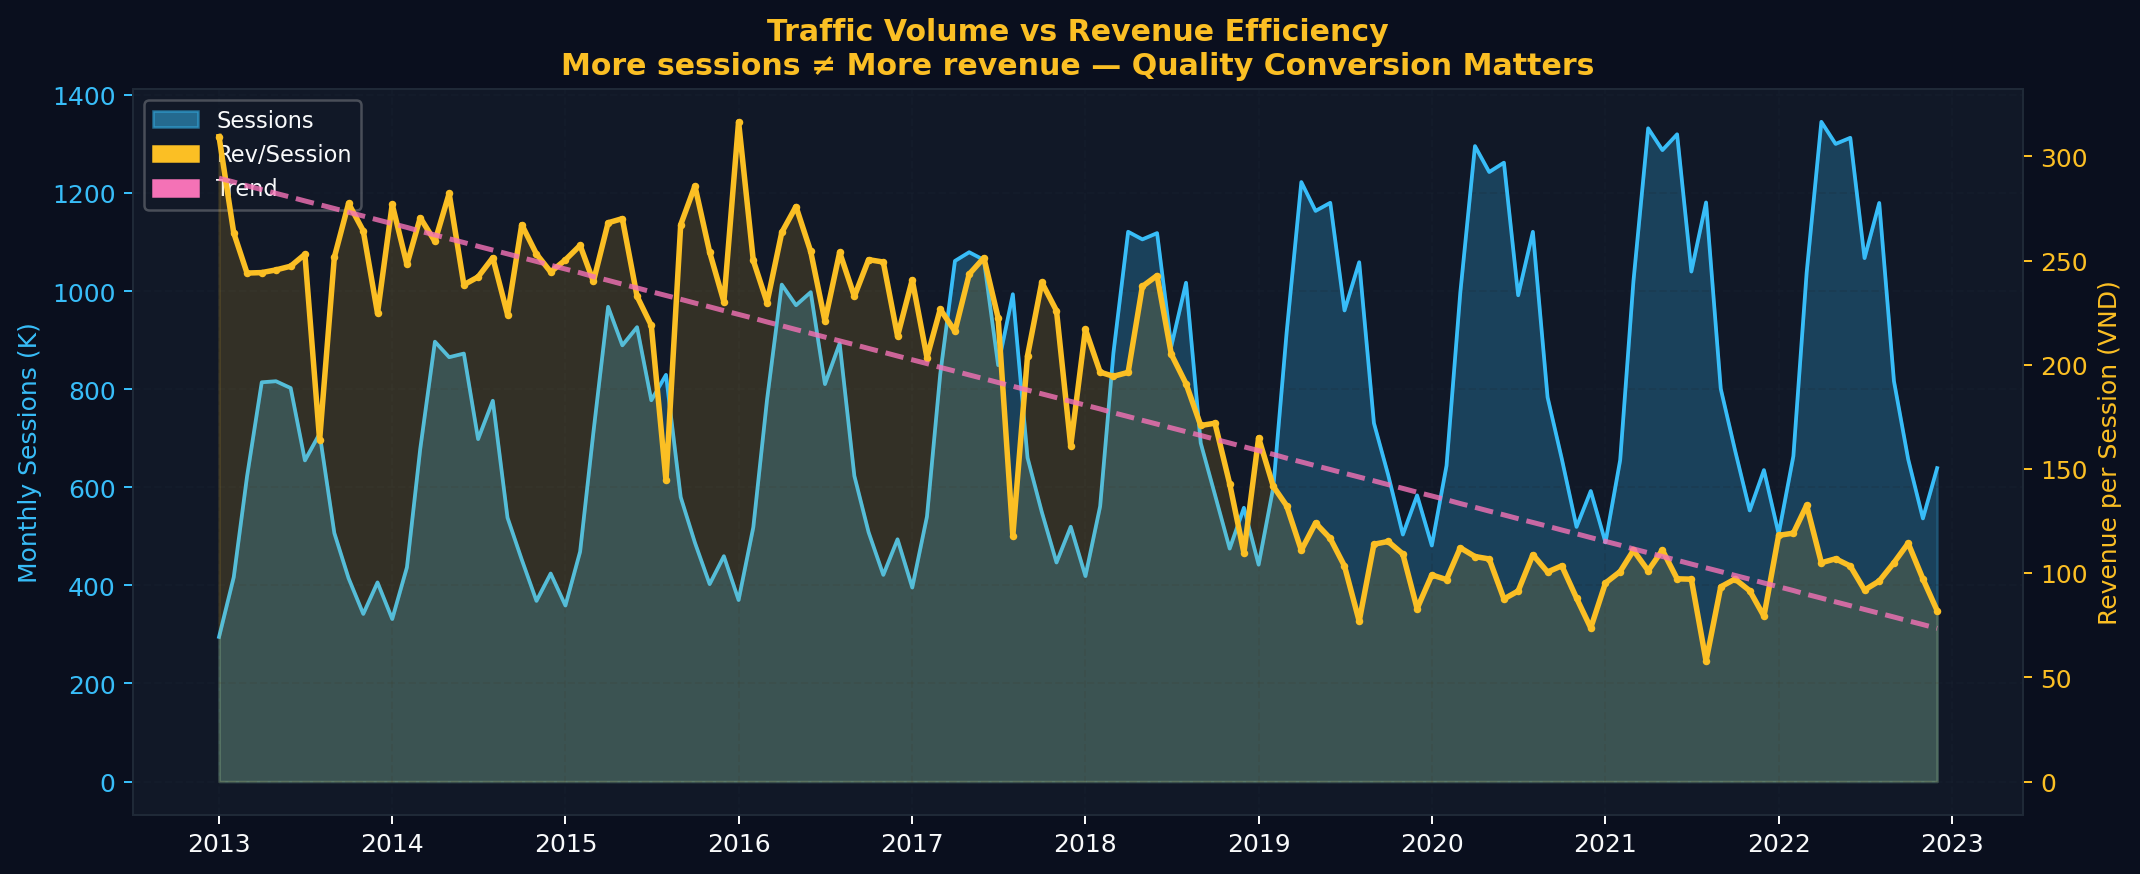
\includegraphics[width=\textwidth]{charts/5b_traffic_efficiency.png}
  \caption{Revenue-per-session declining over time despite session growth.}
  \label{fig:app5b}
\end{figure}

\begin{figure}[htbp]
  \centering
  \begin{subfigure}[t]{0.48\textwidth}
    \centering
    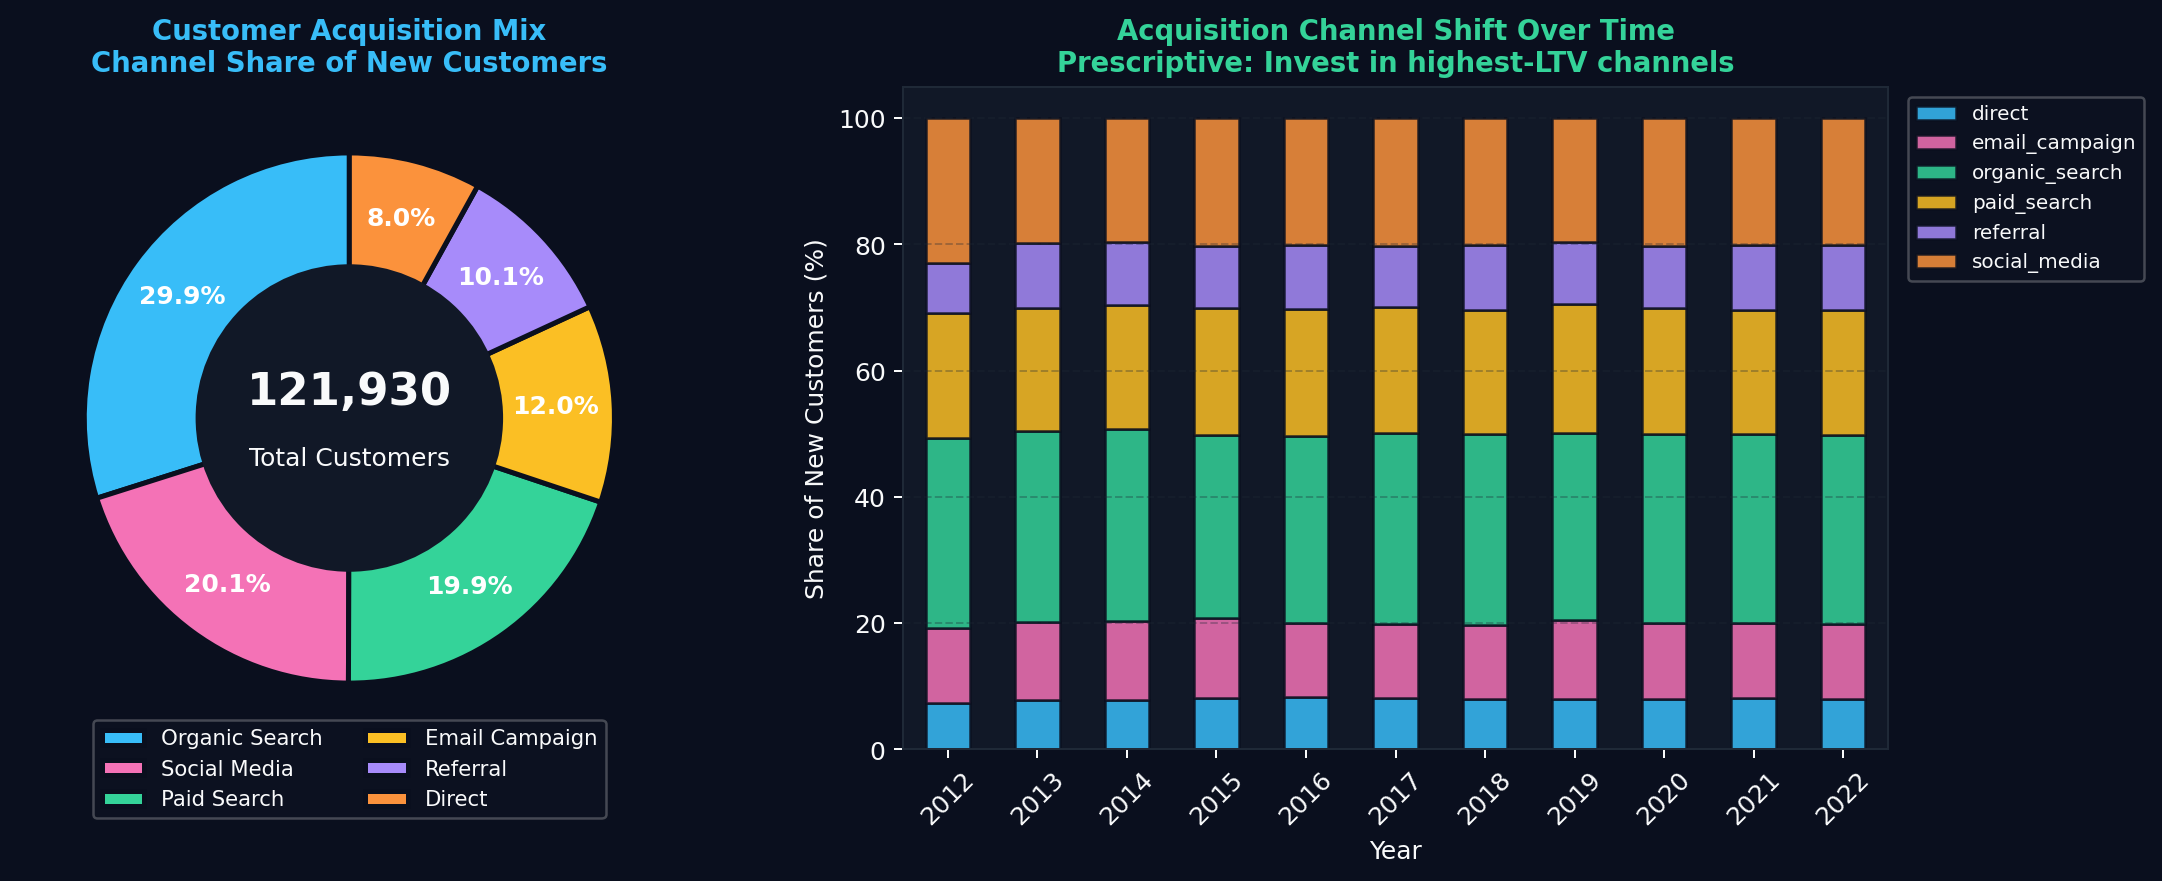
\includegraphics[width=\textwidth]{charts/5c_acquisition_channels.png}
    \caption{Acquisition channel mix evolution.}
    \label{fig:app5c}
  \end{subfigure}\hfill
  \begin{subfigure}[t]{0.48\textwidth}
    \centering
    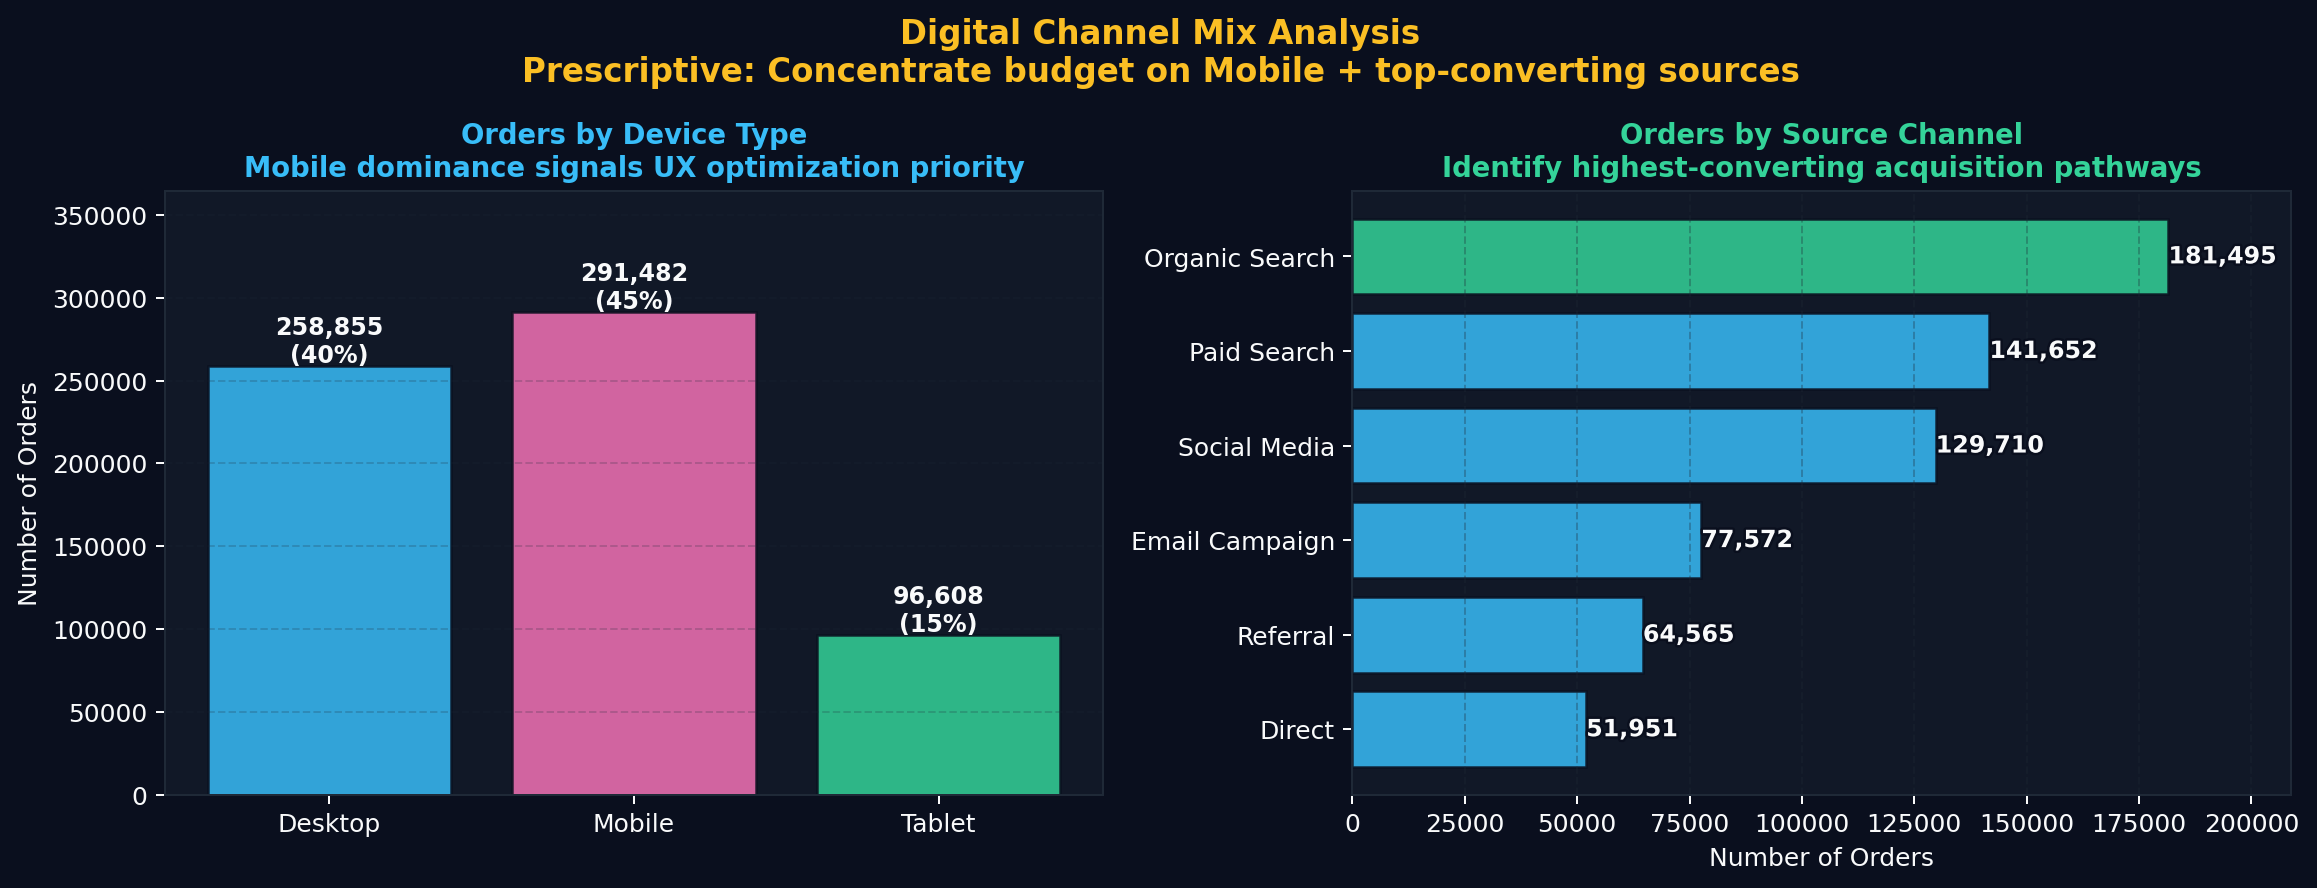
\includegraphics[width=\textwidth]{charts/5d_device_source_orders.png}
    \caption{Mobile leads at 45\% of orders.}
    \label{fig:app5d}
  \end{subfigure}
  \caption{Insight 5 channel and device analysis.}
\end{figure}

\end{document}
